\documentclass[twoside]{book}

% Packages required by doxygen
\usepackage{fixltx2e}
\usepackage{calc}
\usepackage{doxygen}
\usepackage[export]{adjustbox} % also loads graphicx
\usepackage{graphicx}
\usepackage[utf8]{inputenc}
\usepackage{makeidx}
\usepackage{multicol}
\usepackage{multirow}
\PassOptionsToPackage{warn}{textcomp}
\usepackage{textcomp}
\usepackage[nointegrals]{wasysym}
\usepackage[table]{xcolor}

% Font selection
\usepackage[T1]{fontenc}
\usepackage[scaled=.90]{helvet}
\usepackage{courier}
\usepackage{amssymb}
\usepackage{sectsty}
\renewcommand{\familydefault}{\sfdefault}
\allsectionsfont{%
  \fontseries{bc}\selectfont%
  \color{darkgray}%
}
\renewcommand{\DoxyLabelFont}{%
  \fontseries{bc}\selectfont%
  \color{darkgray}%
}
\newcommand{\+}{\discretionary{\mbox{\scriptsize$\hookleftarrow$}}{}{}}

% Page & text layout
\usepackage{geometry}
\geometry{%
  a4paper,%
  top=2.5cm,%
  bottom=2.5cm,%
  left=2.5cm,%
  right=2.5cm%
}
\tolerance=750
\hfuzz=15pt
\hbadness=750
\setlength{\emergencystretch}{15pt}
\setlength{\parindent}{0cm}
\setlength{\parskip}{3ex plus 2ex minus 2ex}
\makeatletter
\renewcommand{\paragraph}{%
  \@startsection{paragraph}{4}{0ex}{-1.0ex}{1.0ex}{%
    \normalfont\normalsize\bfseries\SS@parafont%
  }%
}
\renewcommand{\subparagraph}{%
  \@startsection{subparagraph}{5}{0ex}{-1.0ex}{1.0ex}{%
    \normalfont\normalsize\bfseries\SS@subparafont%
  }%
}
\makeatother

% Headers & footers
\usepackage{fancyhdr}
\pagestyle{fancyplain}
\fancyhead[LE]{\fancyplain{}{\bfseries\thepage}}
\fancyhead[CE]{\fancyplain{}{}}
\fancyhead[RE]{\fancyplain{}{\bfseries\leftmark}}
\fancyhead[LO]{\fancyplain{}{\bfseries\rightmark}}
\fancyhead[CO]{\fancyplain{}{}}
\fancyhead[RO]{\fancyplain{}{\bfseries\thepage}}
\fancyfoot[LE]{\fancyplain{}{}}
\fancyfoot[CE]{\fancyplain{}{}}
\fancyfoot[RE]{\fancyplain{}{\bfseries\scriptsize Generated by Doxygen }}
\fancyfoot[LO]{\fancyplain{}{\bfseries\scriptsize Generated by Doxygen }}
\fancyfoot[CO]{\fancyplain{}{}}
\fancyfoot[RO]{\fancyplain{}{}}
\renewcommand{\footrulewidth}{0.4pt}
\renewcommand{\chaptermark}[1]{%
  \markboth{#1}{}%
}
\renewcommand{\sectionmark}[1]{%
  \markright{\thesection\ #1}%
}

% Indices & bibliography
\usepackage{natbib}
\usepackage[titles]{tocloft}
\setcounter{tocdepth}{3}
\setcounter{secnumdepth}{5}
\makeindex

% Hyperlinks (required, but should be loaded last)
\usepackage{ifpdf}
\ifpdf
  \usepackage[pdftex,pagebackref=true]{hyperref}
\else
  \usepackage[ps2pdf,pagebackref=true]{hyperref}
\fi
\hypersetup{%
  colorlinks=true,%
  linkcolor=blue,%
  citecolor=blue,%
  unicode%
}

% Custom commands
\newcommand{\clearemptydoublepage}{%
  \newpage{\pagestyle{empty}\cleardoublepage}%
}

\usepackage{caption}
\captionsetup{labelsep=space,justification=centering,font={bf},singlelinecheck=off,skip=4pt,position=top}

%===== C O N T E N T S =====

\begin{document}

% Titlepage & ToC
\hypersetup{pageanchor=false,
             bookmarksnumbered=true,
             pdfencoding=unicode
            }
\pagenumbering{alph}
\begin{titlepage}
\vspace*{7cm}
\begin{center}%
{\Large C\+AL Project -\/ Bike Sharing }\\
\vspace*{1cm}
{\large Generated by Doxygen 1.8.14}\\
\end{center}
\end{titlepage}
\clearemptydoublepage
\pagenumbering{roman}
\tableofcontents
\clearemptydoublepage
\pagenumbering{arabic}
\hypersetup{pageanchor=true}

%--- Begin generated contents ---
\chapter{Module Index}
\section{Modules}
Here is a list of all modules\+:\begin{DoxyCompactList}
\item \contentsline{section}{Utilities}{\pageref{group___utilities}}{}
\end{DoxyCompactList}

\chapter{Hierarchical Index}
\section{Class Hierarchy}
This inheritance list is sorted roughly, but not completely, alphabetically\+:\begin{DoxyCompactList}
\item \contentsline{section}{Bike\+Company}{\pageref{class_bike_company}}{}
\item \contentsline{section}{Connection}{\pageref{class_connection}}{}
\item \contentsline{section}{Edge$<$ T $>$}{\pageref{class_edge}}{}
\item \contentsline{section}{Edge\+Type}{\pageref{class_edge_type}}{}
\item \contentsline{section}{Graph$<$ T $>$}{\pageref{class_graph}}{}
\item \contentsline{section}{Graph$<$ Node $>$}{\pageref{class_graph}}{}
\item \contentsline{section}{Graph\+Viewer}{\pageref{class_graph_viewer}}{}
\item \contentsline{section}{Invalid\+Format}{\pageref{class_invalid_format}}{}
\item \contentsline{section}{Mutable\+Priority\+Queue$<$ T $>$}{\pageref{class_mutable_priority_queue}}{}
\item \contentsline{section}{Node}{\pageref{class_node}}{}
\begin{DoxyCompactList}
\item \contentsline{section}{Sharing\+Spot}{\pageref{class_sharing_spot}}{}
\end{DoxyCompactList}
\item \contentsline{section}{Parser}{\pageref{class_parser}}{}
\item \contentsline{section}{Street}{\pageref{class_street}}{}
\item \contentsline{section}{User}{\pageref{class_user}}{}
\item \contentsline{section}{Vertex$<$ T $>$}{\pageref{class_vertex}}{}
\end{DoxyCompactList}

\chapter{Class Index}
\section{Class List}
Here are the classes, structs, unions and interfaces with brief descriptions\+:\begin{DoxyCompactList}
\item\contentsline{section}{\mbox{\hyperlink{class_bike_company}{Bike\+Company}} }{\pageref{class_bike_company}}{}
\item\contentsline{section}{\mbox{\hyperlink{class_connection}{Connection}} }{\pageref{class_connection}}{}
\item\contentsline{section}{\mbox{\hyperlink{class_edge}{Edge$<$ T $>$}} }{\pageref{class_edge}}{}
\item\contentsline{section}{\mbox{\hyperlink{class_edge_type}{Edge\+Type}} }{\pageref{class_edge_type}}{}
\item\contentsline{section}{\mbox{\hyperlink{class_graph}{Graph$<$ T $>$}} }{\pageref{class_graph}}{}
\item\contentsline{section}{\mbox{\hyperlink{class_graph_viewer}{Graph\+Viewer}} }{\pageref{class_graph_viewer}}{}
\item\contentsline{section}{\mbox{\hyperlink{class_invalid_format}{Invalid\+Format}} }{\pageref{class_invalid_format}}{}
\item\contentsline{section}{\mbox{\hyperlink{class_mutable_priority_queue}{Mutable\+Priority\+Queue$<$ T $>$}} }{\pageref{class_mutable_priority_queue}}{}
\item\contentsline{section}{\mbox{\hyperlink{class_node}{Node}} }{\pageref{class_node}}{}
\item\contentsline{section}{\mbox{\hyperlink{class_parser}{Parser}} }{\pageref{class_parser}}{}
\item\contentsline{section}{\mbox{\hyperlink{class_sharing_spot}{Sharing\+Spot}} }{\pageref{class_sharing_spot}}{}
\item\contentsline{section}{\mbox{\hyperlink{class_street}{Street}} }{\pageref{class_street}}{}
\item\contentsline{section}{\mbox{\hyperlink{class_user}{User}} }{\pageref{class_user}}{}
\item\contentsline{section}{\mbox{\hyperlink{class_vertex}{Vertex$<$ T $>$}} }{\pageref{class_vertex}}{}
\end{DoxyCompactList}

\chapter{Module Documentation}
\hypertarget{group___utilities}{}\section{Utilities}
\label{group___utilities}\index{Utilities@{Utilities}}


Utilities is a namespace created to contain useful functions.  




\subsection{Detailed Description}
Utilities is a namespace created to contain useful functions. 


\chapter{Class Documentation}
\hypertarget{class_bike_company}{}\section{Bike\+Company Class Reference}
\label{class_bike_company}\index{Bike\+Company@{Bike\+Company}}
\subsection*{Public Member Functions}
\begin{DoxyCompactItemize}
\item 
\mbox{\hyperlink{class_bike_company_ab435a4495b3ae8602162a51ebf50a3f4}{Bike\+Company}} (const vector$<$ \mbox{\hyperlink{class_node}{Node}} $>$ \&nodes, const vector$<$ \mbox{\hyperlink{class_street}{Street}} $>$ \&streets, const vector$<$ \mbox{\hyperlink{class_sharing_spot}{Sharing\+Spot}} $>$ \&sharing\+Spots, const \mbox{\hyperlink{class_user}{User}} \&user)
\item 
void \mbox{\hyperlink{class_bike_company_ace655ae1ace35afcb0acb4ae842215df}{create\+Graph}} ()
\item 
\mbox{\hyperlink{class_graph_viewer}{Graph\+Viewer}} $\ast$ \mbox{\hyperlink{class_bike_company_a5cdaee132eda4772a117b7f36cb94de3}{print\+Graph}} ()
\item 
void \mbox{\hyperlink{class_bike_company_ae7994d9db29de7064da710915662bd0b}{get\+Nearest\+Sharing\+Spot}} (const \mbox{\hyperlink{class_node}{Node}} \&current\+Position)
\item 
\mbox{\hyperlink{class_graph}{Graph}}$<$ \mbox{\hyperlink{class_node}{Node}} $>$ \& \mbox{\hyperlink{class_bike_company_ab60253ec9b0bb46f913609a189df4cb8}{get\+Graph}} ()
\item 
vector$<$ \mbox{\hyperlink{class_node}{Node}} $>$ \& \mbox{\hyperlink{class_bike_company_ae41458919c4daf896b12960c2b43d51c}{get\+Nodes}} ()
\item 
vector$<$ \mbox{\hyperlink{class_street}{Street}} $>$ \& \mbox{\hyperlink{class_bike_company_a545b86c3c1dbde4b8f70871b4d23be2b}{get\+Streets}} ()
\item 
vector$<$ \mbox{\hyperlink{class_sharing_spot}{Sharing\+Spot}} $>$ \& \mbox{\hyperlink{class_bike_company_ac361f971df61155a1763c682b28f6297}{get\+Sharing\+Spots}} ()
\item 
\mbox{\hyperlink{class_user}{User}} \mbox{\hyperlink{class_bike_company_a19f8b3503630ec5f5c12ead35cdbe995}{get\+User}} ()
\item 
int \mbox{\hyperlink{class_bike_company_a70a2863261f0b9b2087c2ed012a17434}{find\+Street\+By\+Nodes}} (int node\+Id1, int node\+Id2)
\item 
\mbox{\hyperlink{class_street}{Street}} \& \mbox{\hyperlink{class_bike_company_a17955d80bd12b199559b72be003f601a}{find\+Street}} (unsigned long long int id)
\item 
\mbox{\hyperlink{class_node}{Node}} \& \mbox{\hyperlink{class_bike_company_ac3a38462c549de8c3c58c83c5e6f6696}{find\+Node}} (unsigned long long int id)
\item 
\mbox{\hyperlink{class_node}{Node}} \& \mbox{\hyperlink{class_bike_company_a7adfcf36f3e55f8c3498c4b304a3d4dc}{find\+Node\+By\+Id}} (unsigned int id)
\item 
\mbox{\hyperlink{class_node}{Node}} \mbox{\hyperlink{class_bike_company_aa14daa601b5b33e0f4bd3c78a1ff92b8}{get\+Center}} ()
\item 
void \mbox{\hyperlink{class_bike_company_a6cfdaa4ec2d86097301e0aa6f00fff7e}{get\+Cheapest\+Sharing\+Spot}} (const \mbox{\hyperlink{class_node}{Node}} \&current\+Position)
\item 
void \mbox{\hyperlink{class_bike_company_a5619c7888aed213bee9acf09f80fbad8}{check\+Connectivity}} ()
\item 
int \mbox{\hyperlink{class_bike_company_a7c844e84c41eff544d58c6b964dcacf7}{exact\+Search\+Street}} (string street\+Name)
\item 
void \mbox{\hyperlink{class_bike_company_a626158626f8a845c8002731d74231a42}{check\+Existence\+Sharing\+Spot}} (int street\+Id1, int street\+Id2)
\item 
vector$<$ int $>$ \mbox{\hyperlink{class_bike_company_acfc5f830f69bfb5f9db3f41391a1038c}{approximate\+Search\+Street}} (string street\+Name)
\end{DoxyCompactItemize}


\subsection{Constructor \& Destructor Documentation}
\mbox{\Hypertarget{class_bike_company_ab435a4495b3ae8602162a51ebf50a3f4}\label{class_bike_company_ab435a4495b3ae8602162a51ebf50a3f4}} 
\index{Bike\+Company@{Bike\+Company}!Bike\+Company@{Bike\+Company}}
\index{Bike\+Company@{Bike\+Company}!Bike\+Company@{Bike\+Company}}
\subsubsection{\texorpdfstring{Bike\+Company()}{BikeCompany()}}
{\footnotesize\ttfamily Bike\+Company\+::\+Bike\+Company (\begin{DoxyParamCaption}\item[{const vector$<$ \mbox{\hyperlink{class_node}{Node}} $>$ \&}]{nodes,  }\item[{const vector$<$ \mbox{\hyperlink{class_street}{Street}} $>$ \&}]{streets,  }\item[{const vector$<$ \mbox{\hyperlink{class_sharing_spot}{Sharing\+Spot}} $>$ \&}]{sharing\+Spots,  }\item[{const \mbox{\hyperlink{class_user}{User}} \&}]{user }\end{DoxyParamCaption})}

\mbox{\hyperlink{class_bike_company}{Bike\+Company}} constructor 
\begin{DoxyParams}{Parameters}
{\em nodes} & vector with all the nodes from the files (not filtered) \\
\hline
{\em streets} & vector with all the streets from the files (not filtered) \\
\hline
{\em sharing\+Spots} & vector with all the sharing spots (some of the nodes that were chosen) \\
\hline
{\em user} & user information \\
\hline
\end{DoxyParams}


\subsection{Member Function Documentation}
\mbox{\Hypertarget{class_bike_company_acfc5f830f69bfb5f9db3f41391a1038c}\label{class_bike_company_acfc5f830f69bfb5f9db3f41391a1038c}} 
\index{Bike\+Company@{Bike\+Company}!approximate\+Search\+Street@{approximate\+Search\+Street}}
\index{approximate\+Search\+Street@{approximate\+Search\+Street}!Bike\+Company@{Bike\+Company}}
\subsubsection{\texorpdfstring{approximate\+Search\+Street()}{approximateSearchStreet()}}
{\footnotesize\ttfamily vector$<$ int $>$ Bike\+Company\+::approximate\+Search\+Street (\begin{DoxyParamCaption}\item[{string}]{street\+Name }\end{DoxyParamCaption})}

Searches in vector \textquotesingle{}streets\textquotesingle{} and prints the 3 street names more similar with street\+Name. 
\begin{DoxyParams}{Parameters}
{\em street\+Name} & name of the street. \\
\hline
\end{DoxyParams}
\begin{DoxyReturn}{Returns}
vector with the id of the streets displayed. 
\end{DoxyReturn}
\mbox{\Hypertarget{class_bike_company_a5619c7888aed213bee9acf09f80fbad8}\label{class_bike_company_a5619c7888aed213bee9acf09f80fbad8}} 
\index{Bike\+Company@{Bike\+Company}!check\+Connectivity@{check\+Connectivity}}
\index{check\+Connectivity@{check\+Connectivity}!Bike\+Company@{Bike\+Company}}
\subsubsection{\texorpdfstring{check\+Connectivity()}{checkConnectivity()}}
{\footnotesize\ttfamily void Bike\+Company\+::check\+Connectivity (\begin{DoxyParamCaption}{ }\end{DoxyParamCaption})}

Check graph\textquotesingle{}s connectivity \mbox{\Hypertarget{class_bike_company_a626158626f8a845c8002731d74231a42}\label{class_bike_company_a626158626f8a845c8002731d74231a42}} 
\index{Bike\+Company@{Bike\+Company}!check\+Existence\+Sharing\+Spot@{check\+Existence\+Sharing\+Spot}}
\index{check\+Existence\+Sharing\+Spot@{check\+Existence\+Sharing\+Spot}!Bike\+Company@{Bike\+Company}}
\subsubsection{\texorpdfstring{check\+Existence\+Sharing\+Spot()}{checkExistenceSharingSpot()}}
{\footnotesize\ttfamily void Bike\+Company\+::check\+Existence\+Sharing\+Spot (\begin{DoxyParamCaption}\item[{int}]{street\+Id1,  }\item[{int}]{street\+Id2 }\end{DoxyParamCaption})}

Checks if there is a sharing spot in the intersection between the streets given as parameters. 
\begin{DoxyParams}{Parameters}
{\em street\+Id1} & id of street 1. \\
\hline
{\em street\+Id2} & id of street 2. \\
\hline
\end{DoxyParams}
\mbox{\Hypertarget{class_bike_company_ace655ae1ace35afcb0acb4ae842215df}\label{class_bike_company_ace655ae1ace35afcb0acb4ae842215df}} 
\index{Bike\+Company@{Bike\+Company}!create\+Graph@{create\+Graph}}
\index{create\+Graph@{create\+Graph}!Bike\+Company@{Bike\+Company}}
\subsubsection{\texorpdfstring{create\+Graph()}{createGraph()}}
{\footnotesize\ttfamily void Bike\+Company\+::create\+Graph (\begin{DoxyParamCaption}{ }\end{DoxyParamCaption})}

Fills graph with the vertexs and the edges \mbox{\Hypertarget{class_bike_company_a7c844e84c41eff544d58c6b964dcacf7}\label{class_bike_company_a7c844e84c41eff544d58c6b964dcacf7}} 
\index{Bike\+Company@{Bike\+Company}!exact\+Search\+Street@{exact\+Search\+Street}}
\index{exact\+Search\+Street@{exact\+Search\+Street}!Bike\+Company@{Bike\+Company}}
\subsubsection{\texorpdfstring{exact\+Search\+Street()}{exactSearchStreet()}}
{\footnotesize\ttfamily int Bike\+Company\+::exact\+Search\+Street (\begin{DoxyParamCaption}\item[{string}]{street\+Name }\end{DoxyParamCaption})}

Searches in vector \textquotesingle{}streets\textquotesingle{} if there is an exact match with street\+Name. 
\begin{DoxyParams}{Parameters}
{\em street\+Name} & name of street. \\
\hline
\end{DoxyParams}
\begin{DoxyReturn}{Returns}
-\/1 if the street is not found, otherwise returns the street\textquotesingle{}s id. 
\end{DoxyReturn}
\mbox{\Hypertarget{class_bike_company_ac3a38462c549de8c3c58c83c5e6f6696}\label{class_bike_company_ac3a38462c549de8c3c58c83c5e6f6696}} 
\index{Bike\+Company@{Bike\+Company}!find\+Node@{find\+Node}}
\index{find\+Node@{find\+Node}!Bike\+Company@{Bike\+Company}}
\subsubsection{\texorpdfstring{find\+Node()}{findNode()}}
{\footnotesize\ttfamily \mbox{\hyperlink{class_node}{Node}} \& Bike\+Company\+::find\+Node (\begin{DoxyParamCaption}\item[{unsigned long long int}]{id }\end{DoxyParamCaption})}

Finds the node with the specified open street map id 
\begin{DoxyParams}{Parameters}
{\em id} & node id \\
\hline
\end{DoxyParams}
\begin{DoxyReturn}{Returns}
node 
\end{DoxyReturn}
\mbox{\Hypertarget{class_bike_company_a7adfcf36f3e55f8c3498c4b304a3d4dc}\label{class_bike_company_a7adfcf36f3e55f8c3498c4b304a3d4dc}} 
\index{Bike\+Company@{Bike\+Company}!find\+Node\+By\+Id@{find\+Node\+By\+Id}}
\index{find\+Node\+By\+Id@{find\+Node\+By\+Id}!Bike\+Company@{Bike\+Company}}
\subsubsection{\texorpdfstring{find\+Node\+By\+Id()}{findNodeById()}}
{\footnotesize\ttfamily \mbox{\hyperlink{class_node}{Node}} \& Bike\+Company\+::find\+Node\+By\+Id (\begin{DoxyParamCaption}\item[{unsigned int}]{id }\end{DoxyParamCaption})}

Finds the node with the specified id 
\begin{DoxyParams}{Parameters}
{\em id} & node id \\
\hline
\end{DoxyParams}
\begin{DoxyReturn}{Returns}
node 
\end{DoxyReturn}
\mbox{\Hypertarget{class_bike_company_a17955d80bd12b199559b72be003f601a}\label{class_bike_company_a17955d80bd12b199559b72be003f601a}} 
\index{Bike\+Company@{Bike\+Company}!find\+Street@{find\+Street}}
\index{find\+Street@{find\+Street}!Bike\+Company@{Bike\+Company}}
\subsubsection{\texorpdfstring{find\+Street()}{findStreet()}}
{\footnotesize\ttfamily \mbox{\hyperlink{class_street}{Street}} \& Bike\+Company\+::find\+Street (\begin{DoxyParamCaption}\item[{unsigned long long int}]{id }\end{DoxyParamCaption})}

Finds the street with the specified if 
\begin{DoxyParams}{Parameters}
{\em id} & street id \\
\hline
\end{DoxyParams}
\begin{DoxyReturn}{Returns}
street 
\end{DoxyReturn}
\mbox{\Hypertarget{class_bike_company_a70a2863261f0b9b2087c2ed012a17434}\label{class_bike_company_a70a2863261f0b9b2087c2ed012a17434}} 
\index{Bike\+Company@{Bike\+Company}!find\+Street\+By\+Nodes@{find\+Street\+By\+Nodes}}
\index{find\+Street\+By\+Nodes@{find\+Street\+By\+Nodes}!Bike\+Company@{Bike\+Company}}
\subsubsection{\texorpdfstring{find\+Street\+By\+Nodes()}{findStreetByNodes()}}
{\footnotesize\ttfamily int Bike\+Company\+::find\+Street\+By\+Nodes (\begin{DoxyParamCaption}\item[{int}]{node\+Id1,  }\item[{int}]{node\+Id2 }\end{DoxyParamCaption})}

Finds a street that starts in node\+Id1 and ends in node\+Id2


\begin{DoxyParams}{Parameters}
{\em node\+Id1} & initial node \\
\hline
{\em node\+Id2} & final node \\
\hline
\end{DoxyParams}
\begin{DoxyReturn}{Returns}
id of the street, or -\/1 if no street is found 
\end{DoxyReturn}
\mbox{\Hypertarget{class_bike_company_aa14daa601b5b33e0f4bd3c78a1ff92b8}\label{class_bike_company_aa14daa601b5b33e0f4bd3c78a1ff92b8}} 
\index{Bike\+Company@{Bike\+Company}!get\+Center@{get\+Center}}
\index{get\+Center@{get\+Center}!Bike\+Company@{Bike\+Company}}
\subsubsection{\texorpdfstring{get\+Center()}{getCenter()}}
{\footnotesize\ttfamily \mbox{\hyperlink{class_node}{Node}} Bike\+Company\+::get\+Center (\begin{DoxyParamCaption}{ }\end{DoxyParamCaption})}

Returns a node that identifies the center of the graph \begin{DoxyReturn}{Returns}
center node 
\end{DoxyReturn}
\mbox{\Hypertarget{class_bike_company_a6cfdaa4ec2d86097301e0aa6f00fff7e}\label{class_bike_company_a6cfdaa4ec2d86097301e0aa6f00fff7e}} 
\index{Bike\+Company@{Bike\+Company}!get\+Cheapest\+Sharing\+Spot@{get\+Cheapest\+Sharing\+Spot}}
\index{get\+Cheapest\+Sharing\+Spot@{get\+Cheapest\+Sharing\+Spot}!Bike\+Company@{Bike\+Company}}
\subsubsection{\texorpdfstring{get\+Cheapest\+Sharing\+Spot()}{getCheapestSharingSpot()}}
{\footnotesize\ttfamily void Bike\+Company\+::get\+Cheapest\+Sharing\+Spot (\begin{DoxyParamCaption}\item[{const \mbox{\hyperlink{class_node}{Node}} \&}]{current\+Position }\end{DoxyParamCaption})}

Finds the cheapest sharing spot and calls function to draw path to it. 
\begin{DoxyParams}{Parameters}
{\em current\+Position} & user\textquotesingle{}s current position \\
\hline
\end{DoxyParams}
\mbox{\Hypertarget{class_bike_company_ab60253ec9b0bb46f913609a189df4cb8}\label{class_bike_company_ab60253ec9b0bb46f913609a189df4cb8}} 
\index{Bike\+Company@{Bike\+Company}!get\+Graph@{get\+Graph}}
\index{get\+Graph@{get\+Graph}!Bike\+Company@{Bike\+Company}}
\subsubsection{\texorpdfstring{get\+Graph()}{getGraph()}}
{\footnotesize\ttfamily \mbox{\hyperlink{class_graph}{Graph}}$<$\mbox{\hyperlink{class_node}{Node}}$>$\& Bike\+Company\+::get\+Graph (\begin{DoxyParamCaption}{ }\end{DoxyParamCaption})\hspace{0.3cm}{\ttfamily [inline]}}

Getter which returns the graph \begin{DoxyReturn}{Returns}
graph 
\end{DoxyReturn}
\mbox{\Hypertarget{class_bike_company_ae7994d9db29de7064da710915662bd0b}\label{class_bike_company_ae7994d9db29de7064da710915662bd0b}} 
\index{Bike\+Company@{Bike\+Company}!get\+Nearest\+Sharing\+Spot@{get\+Nearest\+Sharing\+Spot}}
\index{get\+Nearest\+Sharing\+Spot@{get\+Nearest\+Sharing\+Spot}!Bike\+Company@{Bike\+Company}}
\subsubsection{\texorpdfstring{get\+Nearest\+Sharing\+Spot()}{getNearestSharingSpot()}}
{\footnotesize\ttfamily void Bike\+Company\+::get\+Nearest\+Sharing\+Spot (\begin{DoxyParamCaption}\item[{const \mbox{\hyperlink{class_node}{Node}} \&}]{current\+Position }\end{DoxyParamCaption})}

Finds the nearest sharing spot and calls function to draw path to it. 
\begin{DoxyParams}{Parameters}
{\em current\+Position} & user\textquotesingle{}s current position \\
\hline
\end{DoxyParams}
\mbox{\Hypertarget{class_bike_company_ae41458919c4daf896b12960c2b43d51c}\label{class_bike_company_ae41458919c4daf896b12960c2b43d51c}} 
\index{Bike\+Company@{Bike\+Company}!get\+Nodes@{get\+Nodes}}
\index{get\+Nodes@{get\+Nodes}!Bike\+Company@{Bike\+Company}}
\subsubsection{\texorpdfstring{get\+Nodes()}{getNodes()}}
{\footnotesize\ttfamily vector$<$\mbox{\hyperlink{class_node}{Node}}$>$\& Bike\+Company\+::get\+Nodes (\begin{DoxyParamCaption}{ }\end{DoxyParamCaption})\hspace{0.3cm}{\ttfamily [inline]}}

Getter which returns a vector with all the nodes \begin{DoxyReturn}{Returns}
vector with all the nodes 
\end{DoxyReturn}
\mbox{\Hypertarget{class_bike_company_ac361f971df61155a1763c682b28f6297}\label{class_bike_company_ac361f971df61155a1763c682b28f6297}} 
\index{Bike\+Company@{Bike\+Company}!get\+Sharing\+Spots@{get\+Sharing\+Spots}}
\index{get\+Sharing\+Spots@{get\+Sharing\+Spots}!Bike\+Company@{Bike\+Company}}
\subsubsection{\texorpdfstring{get\+Sharing\+Spots()}{getSharingSpots()}}
{\footnotesize\ttfamily vector$<$\mbox{\hyperlink{class_sharing_spot}{Sharing\+Spot}}$>$\& Bike\+Company\+::get\+Sharing\+Spots (\begin{DoxyParamCaption}{ }\end{DoxyParamCaption})\hspace{0.3cm}{\ttfamily [inline]}}

Getter which returns a vector with all the sharing spots \begin{DoxyReturn}{Returns}
vector with all the sharing spots 
\end{DoxyReturn}
\mbox{\Hypertarget{class_bike_company_a545b86c3c1dbde4b8f70871b4d23be2b}\label{class_bike_company_a545b86c3c1dbde4b8f70871b4d23be2b}} 
\index{Bike\+Company@{Bike\+Company}!get\+Streets@{get\+Streets}}
\index{get\+Streets@{get\+Streets}!Bike\+Company@{Bike\+Company}}
\subsubsection{\texorpdfstring{get\+Streets()}{getStreets()}}
{\footnotesize\ttfamily vector$<$\mbox{\hyperlink{class_street}{Street}}$>$\& Bike\+Company\+::get\+Streets (\begin{DoxyParamCaption}{ }\end{DoxyParamCaption})\hspace{0.3cm}{\ttfamily [inline]}}

Getter which returns a vector with all the streets \begin{DoxyReturn}{Returns}
vector with all the streets 
\end{DoxyReturn}
\mbox{\Hypertarget{class_bike_company_a19f8b3503630ec5f5c12ead35cdbe995}\label{class_bike_company_a19f8b3503630ec5f5c12ead35cdbe995}} 
\index{Bike\+Company@{Bike\+Company}!get\+User@{get\+User}}
\index{get\+User@{get\+User}!Bike\+Company@{Bike\+Company}}
\subsubsection{\texorpdfstring{get\+User()}{getUser()}}
{\footnotesize\ttfamily \mbox{\hyperlink{class_user}{User}} Bike\+Company\+::get\+User (\begin{DoxyParamCaption}{ }\end{DoxyParamCaption})\hspace{0.3cm}{\ttfamily [inline]}}

Getter which returns the user information \begin{DoxyReturn}{Returns}
user information 
\end{DoxyReturn}
\mbox{\Hypertarget{class_bike_company_a5cdaee132eda4772a117b7f36cb94de3}\label{class_bike_company_a5cdaee132eda4772a117b7f36cb94de3}} 
\index{Bike\+Company@{Bike\+Company}!print\+Graph@{print\+Graph}}
\index{print\+Graph@{print\+Graph}!Bike\+Company@{Bike\+Company}}
\subsubsection{\texorpdfstring{print\+Graph()}{printGraph()}}
{\footnotesize\ttfamily \mbox{\hyperlink{class_graph_viewer}{Graph\+Viewer}} $\ast$ Bike\+Company\+::print\+Graph (\begin{DoxyParamCaption}{ }\end{DoxyParamCaption})}

Prints graph using \mbox{\hyperlink{class_graph_viewer}{Graph\+Viewer}} 

The documentation for this class was generated from the following files\+:\begin{DoxyCompactItemize}
\item 
src/Bike\+Company.\+h\item 
src/Bike\+Company.\+cpp\end{DoxyCompactItemize}

\hypertarget{class_connection}{}\section{Connection Class Reference}
\label{class_connection}\index{Connection@{Connection}}
\subsection*{Public Member Functions}
\begin{DoxyCompactItemize}
\item 
\mbox{\Hypertarget{class_connection_a8089476d48ba545f44e691cd4bd0278d}\label{class_connection_a8089476d48ba545f44e691cd4bd0278d}} 
{\bfseries Connection} (short port)
\item 
\mbox{\Hypertarget{class_connection_a4b9f6db1fb42fc9857f829fa0bc52e6e}\label{class_connection_a4b9f6db1fb42fc9857f829fa0bc52e6e}} 
bool {\bfseries send\+Msg} (string msg)
\item 
\mbox{\Hypertarget{class_connection_a1df16b436751b686d96c24ca0c498659}\label{class_connection_a1df16b436751b686d96c24ca0c498659}} 
string {\bfseries read\+Line} ()
\end{DoxyCompactItemize}


The documentation for this class was generated from the following files\+:\begin{DoxyCompactItemize}
\item 
src/connection.\+h\item 
src/connection.\+cpp\end{DoxyCompactItemize}

\hypertarget{class_edge}{}\section{Edge$<$ T $>$ Class Template Reference}
\label{class_edge}\index{Edge$<$ T $>$@{Edge$<$ T $>$}}
\subsection*{Public Member Functions}
\begin{DoxyCompactItemize}
\item 
\mbox{\Hypertarget{class_edge_a9da861a03f920c89984be33515a5d870}\label{class_edge_a9da861a03f920c89984be33515a5d870}} 
{\bfseries Edge} (\mbox{\hyperlink{class_vertex}{Vertex}}$<$ T $>$ $\ast$d, double w)
\end{DoxyCompactItemize}
\subsection*{Friends}
\begin{DoxyCompactItemize}
\item 
\mbox{\Hypertarget{class_edge_aefa9b76cd57411c5354e5620dc2d84dd}\label{class_edge_aefa9b76cd57411c5354e5620dc2d84dd}} 
class {\bfseries Graph$<$ T $>$}
\item 
\mbox{\Hypertarget{class_edge_a2e120a12dec663fa334633b4f26cbed8}\label{class_edge_a2e120a12dec663fa334633b4f26cbed8}} 
class {\bfseries Vertex$<$ T $>$}
\end{DoxyCompactItemize}


The documentation for this class was generated from the following file\+:\begin{DoxyCompactItemize}
\item 
src/graph.\+h\end{DoxyCompactItemize}

\hypertarget{class_edge_type}{}\section{Edge\+Type Class Reference}
\label{class_edge_type}\index{Edge\+Type@{Edge\+Type}}


{\ttfamily \#include $<$edgetype.\+h$>$}

\subsection*{Static Public Attributes}
\begin{DoxyCompactItemize}
\item 
\mbox{\Hypertarget{class_edge_type_a6533cc56d05c288a550b9980b66c9317}\label{class_edge_type_a6533cc56d05c288a550b9980b66c9317}} 
static const int {\bfseries U\+N\+D\+I\+R\+E\+C\+T\+ED} = 0
\item 
\mbox{\Hypertarget{class_edge_type_a903017a534f2818c2d17145e4ae0321c}\label{class_edge_type_a903017a534f2818c2d17145e4ae0321c}} 
static const int {\bfseries D\+I\+R\+E\+C\+T\+ED} = 1
\end{DoxyCompactItemize}


\subsection{Detailed Description}
Classe que enumera os tipos de arestas. Usar Edge\+Type.\+U\+N\+D\+I\+R\+E\+C\+T\+ED para uma aresta sem direcção, ou Edge\+Type.\+D\+I\+R\+E\+C\+T\+ED para uma aresta dirigida. 

The documentation for this class was generated from the following file\+:\begin{DoxyCompactItemize}
\item 
src/edgetype.\+h\end{DoxyCompactItemize}

\hypertarget{class_graph}{}\section{Graph$<$ T $>$ Class Template Reference}
\label{class_graph}\index{Graph$<$ T $>$@{Graph$<$ T $>$}}
\subsection*{Public Member Functions}
\begin{DoxyCompactItemize}
\item 
\mbox{\Hypertarget{class_graph_a0853eac15cdf0f06d63f4b8a7820ec71}\label{class_graph_a0853eac15cdf0f06d63f4b8a7820ec71}} 
int {\bfseries get\+Num\+Vertex} () const
\item 
\mbox{\Hypertarget{class_graph_aa81373c1c18aa90c13bea9508f766132}\label{class_graph_aa81373c1c18aa90c13bea9508f766132}} 
vector$<$ \mbox{\hyperlink{class_vertex}{Vertex}}$<$ T $>$ $\ast$ $>$ {\bfseries get\+Vertex\+Set} ()
\item 
\mbox{\Hypertarget{class_graph_a00be284ea2be3b3d0f0d2e493b70245b}\label{class_graph_a00be284ea2be3b3d0f0d2e493b70245b}} 
bool {\bfseries add\+Vertex} (const T \&in)
\item 
\mbox{\Hypertarget{class_graph_af9c903104ad69a7782979fa9caedf163}\label{class_graph_af9c903104ad69a7782979fa9caedf163}} 
bool {\bfseries remove\+Vertex} (const T \&in)
\item 
\mbox{\Hypertarget{class_graph_ac61af3aafe6277215f5a3b3cc7d58ce2}\label{class_graph_ac61af3aafe6277215f5a3b3cc7d58ce2}} 
bool {\bfseries add\+Edge} (const T \&sourc, const T \&dest, double w)
\item 
\mbox{\Hypertarget{class_graph_a1106092a37366486cf55576f9ec01692}\label{class_graph_a1106092a37366486cf55576f9ec01692}} 
bool {\bfseries remove\+Edge} (const T \&sourc, const T \&dest)
\item 
\mbox{\Hypertarget{class_graph_a41afa32aae97b70ecaacabe5fb1a4cf0}\label{class_graph_a41afa32aae97b70ecaacabe5fb1a4cf0}} 
vector$<$ vector$<$ T $>$ $>$ {\bfseries dfs} () const
\item 
\mbox{\Hypertarget{class_graph_aa47a4130165550e208e7a063fce6983a}\label{class_graph_aa47a4130165550e208e7a063fce6983a}} 
vector$<$ T $>$ {\bfseries bfs} (const T \&source) const
\item 
\mbox{\Hypertarget{class_graph_af1d4affd1f886bf598d0f4cf4a0cb7cb}\label{class_graph_af1d4affd1f886bf598d0f4cf4a0cb7cb}} 
vector$<$ T $>$ {\bfseries topsort} () const
\item 
\mbox{\Hypertarget{class_graph_a3dbf946fc46257f2d799077ffba5980f}\label{class_graph_a3dbf946fc46257f2d799077ffba5980f}} 
int {\bfseries max\+New\+Children} (const T \&source, T \&inf) const
\item 
\mbox{\Hypertarget{class_graph_a1ea1512afe5ab878301bc806c2eba9d2}\label{class_graph_a1ea1512afe5ab878301bc806c2eba9d2}} 
bool {\bfseries is\+D\+AG} () const
\item 
\mbox{\hyperlink{class_vertex}{Vertex}}$<$ T $>$ $\ast$ \mbox{\hyperlink{class_graph_ab78574b192c290ede05a031d361b97f9}{init\+Single\+Source}} (const T \&origin)
\item 
bool \mbox{\hyperlink{class_graph_a2cb89dd50ee5fee83ccd9204b80af055}{relax}} (\mbox{\hyperlink{class_vertex}{Vertex}}$<$ T $>$ $\ast$v, \mbox{\hyperlink{class_vertex}{Vertex}}$<$ T $>$ $\ast$w, double weight)
\item 
void \mbox{\hyperlink{class_graph_ac7238d1a3677996b627f8eb1b4300c9e}{dijkstra\+Shortest\+Path}} (const T \&origin)
\item 
\mbox{\Hypertarget{class_graph_a5abed3d7a650413b8197e4662679008d}\label{class_graph_a5abed3d7a650413b8197e4662679008d}} 
vector$<$ T $>$ {\bfseries get\+Path} (const T \&origin, const T \&dest, double \&total\+Weight) const
\end{DoxyCompactItemize}


\subsection{Member Function Documentation}
\mbox{\Hypertarget{class_graph_ac7238d1a3677996b627f8eb1b4300c9e}\label{class_graph_ac7238d1a3677996b627f8eb1b4300c9e}} 
\index{Graph@{Graph}!dijkstra\+Shortest\+Path@{dijkstra\+Shortest\+Path}}
\index{dijkstra\+Shortest\+Path@{dijkstra\+Shortest\+Path}!Graph@{Graph}}
\subsubsection{\texorpdfstring{dijkstra\+Shortest\+Path()}{dijkstraShortestPath()}}
{\footnotesize\ttfamily template$<$class T$>$ \\
void \mbox{\hyperlink{class_graph}{Graph}}$<$ T $>$\+::dijkstra\+Shortest\+Path (\begin{DoxyParamCaption}\item[{const T \&}]{origin }\end{DoxyParamCaption})}

Dijkstra algorithm. \mbox{\Hypertarget{class_graph_ab78574b192c290ede05a031d361b97f9}\label{class_graph_ab78574b192c290ede05a031d361b97f9}} 
\index{Graph@{Graph}!init\+Single\+Source@{init\+Single\+Source}}
\index{init\+Single\+Source@{init\+Single\+Source}!Graph@{Graph}}
\subsubsection{\texorpdfstring{init\+Single\+Source()}{initSingleSource()}}
{\footnotesize\ttfamily template$<$class T$>$ \\
\mbox{\hyperlink{class_vertex}{Vertex}}$<$ T $>$ $\ast$ \mbox{\hyperlink{class_graph}{Graph}}$<$ T $>$\+::init\+Single\+Source (\begin{DoxyParamCaption}\item[{const T \&}]{origin }\end{DoxyParamCaption})}

Initializes single-\/source shortest path data (path, dist). Receives the content of the source vertex and returns a pointer to the source vertex. Used by all single-\/source shortest path algorithms. \mbox{\Hypertarget{class_graph_a2cb89dd50ee5fee83ccd9204b80af055}\label{class_graph_a2cb89dd50ee5fee83ccd9204b80af055}} 
\index{Graph@{Graph}!relax@{relax}}
\index{relax@{relax}!Graph@{Graph}}
\subsubsection{\texorpdfstring{relax()}{relax()}}
{\footnotesize\ttfamily template$<$class T$>$ \\
bool \mbox{\hyperlink{class_graph}{Graph}}$<$ T $>$\+::relax (\begin{DoxyParamCaption}\item[{\mbox{\hyperlink{class_vertex}{Vertex}}$<$ T $>$ $\ast$}]{v,  }\item[{\mbox{\hyperlink{class_vertex}{Vertex}}$<$ T $>$ $\ast$}]{w,  }\item[{double}]{weight }\end{DoxyParamCaption})}

Analyzes an edge in single-\/source shortest path algorithm. Returns true if the target vertex was relaxed (dist, path). Used by all single-\/source shortest path algorithms. 

The documentation for this class was generated from the following file\+:\begin{DoxyCompactItemize}
\item 
src/graph.\+h\end{DoxyCompactItemize}

\hypertarget{class_graph_viewer}{}\section{Graph\+Viewer Class Reference}
\label{class_graph_viewer}\index{Graph\+Viewer@{Graph\+Viewer}}


{\ttfamily \#include $<$graphviewer.\+h$>$}

\subsection*{Public Member Functions}
\begin{DoxyCompactItemize}
\item 
\mbox{\hyperlink{class_graph_viewer_a8adc614f4fc290a3efcec7d7ceb1c58a}{Graph\+Viewer}} (int width, int height, bool dynamic)
\item 
\mbox{\hyperlink{class_graph_viewer_ad9d7b1d8b4ba8ef18517eae0e68568a2}{Graph\+Viewer}} (int width, int height, bool dynamic, int port\+\_\+n)
\item 
bool \mbox{\hyperlink{class_graph_viewer_ae5247dc66449dcd21fc5d531bbbaddfa}{create\+Window}} (int width, int height)
\item 
bool \mbox{\hyperlink{class_graph_viewer_a85990c1eaac7feed3950960d4bd2fd4c}{close\+Window}} ()
\item 
bool \mbox{\hyperlink{class_graph_viewer_a5421e86ac76433876309236ba96e70a2}{add\+Node}} (int id, int x, int y)
\item 
bool \mbox{\hyperlink{class_graph_viewer_ab9be856eb5f45284719a3bb119ec01ea}{add\+Node}} (int id)
\item 
bool \mbox{\hyperlink{class_graph_viewer_aad0c1448c37f744209ffb671f1bd0015}{add\+Edge}} (int id, int v1, int v2, int edge\+Type)
\item 
bool \mbox{\hyperlink{class_graph_viewer_a0c418639bb911eb827cabf895915f775}{remove\+Node}} (int id)
\item 
bool \mbox{\hyperlink{class_graph_viewer_a9a8ee68c7c12b373affbe4069dd95d72}{remove\+Edge}} (int id)
\item 
bool \mbox{\hyperlink{class_graph_viewer_ac25d7d007022fda16799808ba136e909}{set\+Vertex\+Label}} (int id, string label)
\item 
bool \mbox{\hyperlink{class_graph_viewer_a447cca0064e785654c2105602c2961ca}{set\+Edge\+Label}} (int id, string label)
\item 
bool \mbox{\hyperlink{class_graph_viewer_a07ccc96707efae4aa5f3ced3dca015af}{set\+Edge\+Color}} (int id, string color)
\item 
bool \mbox{\hyperlink{class_graph_viewer_a1698f1c6b3a8e7cabc7b7d7cf42fc7f0}{set\+Edge\+Dashed}} (int id, bool dashed)
\item 
bool \mbox{\hyperlink{class_graph_viewer_a8b542d7e09e81a45a74760c19233beb0}{set\+Vertex\+Color}} (int id, string color)
\item 
bool \mbox{\hyperlink{class_graph_viewer_ae930dfdfcdeb7a871eefb6028d74b9f9}{set\+Vertex\+Size}} (int id, int size)
\item 
bool \mbox{\hyperlink{class_graph_viewer_a02d5f7393eab9a2d1b66719039597a64}{set\+Vertex\+Icon}} (int id, string filepath)
\item 
bool \mbox{\hyperlink{class_graph_viewer_a07f598272fe3515455eab13be749604a}{set\+Edge\+Thickness}} (int id, int thickness)
\item 
bool \mbox{\hyperlink{class_graph_viewer_ac211de009a0afe2e6d44f4f8d030a2cc}{set\+Edge\+Weight}} (int id, int weight)
\item 
bool \mbox{\hyperlink{class_graph_viewer_a69eb065145063e4dea41961e92e35c8e}{set\+Edge\+Flow}} (int id, int flow)
\item 
bool \mbox{\hyperlink{class_graph_viewer_a08f362be0e682d91e7506dca8caae1b8}{define\+Edge\+Curved}} (bool curved)
\item 
bool \mbox{\hyperlink{class_graph_viewer_a4102580b69826ba83251ef7bb262f8be}{define\+Edge\+Color}} (string color)
\item 
bool \mbox{\hyperlink{class_graph_viewer_af785279b5c204df0e274b20c36276fc3}{define\+Edge\+Dashed}} (bool dashed)
\item 
bool \mbox{\hyperlink{class_graph_viewer_a76de8676b7a93d72af514b84cdaa4d21}{define\+Vertex\+Color}} (string color)
\item 
bool \mbox{\hyperlink{class_graph_viewer_ac4b2a9fec74d38e64088aa79ca4b7d9b}{define\+Vertex\+Size}} (int size)
\item 
bool \mbox{\hyperlink{class_graph_viewer_af1adb6a361457187a820e01dcf0a34b7}{define\+Vertex\+Icon}} (string filepath)
\item 
bool \mbox{\hyperlink{class_graph_viewer_a02437b5fecd8b90de24436068312d593}{set\+Background}} (string path)
\item 
bool \mbox{\hyperlink{class_graph_viewer_a3009a66958686ccb7e78b68e37c3c423}{rearrange}} ()
\end{DoxyCompactItemize}
\subsection*{Static Public Attributes}
\begin{DoxyCompactItemize}
\item 
static short \mbox{\hyperlink{class_graph_viewer_a89d0abe75f41feededc49497cc514342}{port}} = 7772
\end{DoxyCompactItemize}


\subsection{Detailed Description}
Classe que guarda o grafo e o representa. Todas as suas funções retornam um booleano a indicar se a sua execução decorreu ou não com sucesso. 

\subsection{Constructor \& Destructor Documentation}
\mbox{\Hypertarget{class_graph_viewer_a8adc614f4fc290a3efcec7d7ceb1c58a}\label{class_graph_viewer_a8adc614f4fc290a3efcec7d7ceb1c58a}} 
\index{Graph\+Viewer@{Graph\+Viewer}!Graph\+Viewer@{Graph\+Viewer}}
\index{Graph\+Viewer@{Graph\+Viewer}!Graph\+Viewer@{Graph\+Viewer}}
\subsubsection{\texorpdfstring{Graph\+Viewer()}{GraphViewer()}\hspace{0.1cm}{\footnotesize\ttfamily [1/2]}}
{\footnotesize\ttfamily Graph\+Viewer\+::\+Graph\+Viewer (\begin{DoxyParamCaption}\item[{int}]{width,  }\item[{int}]{height,  }\item[{bool}]{dynamic }\end{DoxyParamCaption})}

Construtor que cria um novo grafo e atribui automaticamente a porta. Exemplo\+: \mbox{\hyperlink{class_graph_viewer}{Graph\+Viewer}} $\ast$gv = new \mbox{\hyperlink{class_graph_viewer}{Graph\+Viewer(600, 600, true)}}; instancia um grafo 600x600, onde a posição dos nós é determinada automaticamente.


\begin{DoxyParams}{Parameters}
{\em width} & Inteiro que representa a lagura da área do grafo. \\
\hline
{\em height} & Inteiro que representa a altura da área do grafo. \\
\hline
{\em dynamic} & Booleano que determina se a localização dos nós é automaticamente. determinado pelo programa (true) ou se deve ser determinado pelo utilizador (false). \\
\hline
\end{DoxyParams}
\mbox{\Hypertarget{class_graph_viewer_ad9d7b1d8b4ba8ef18517eae0e68568a2}\label{class_graph_viewer_ad9d7b1d8b4ba8ef18517eae0e68568a2}} 
\index{Graph\+Viewer@{Graph\+Viewer}!Graph\+Viewer@{Graph\+Viewer}}
\index{Graph\+Viewer@{Graph\+Viewer}!Graph\+Viewer@{Graph\+Viewer}}
\subsubsection{\texorpdfstring{Graph\+Viewer()}{GraphViewer()}\hspace{0.1cm}{\footnotesize\ttfamily [2/2]}}
{\footnotesize\ttfamily Graph\+Viewer\+::\+Graph\+Viewer (\begin{DoxyParamCaption}\item[{int}]{width,  }\item[{int}]{height,  }\item[{bool}]{dynamic,  }\item[{int}]{port\+\_\+n }\end{DoxyParamCaption})}

Construtor que cria um novo grafo, utilizando uma porta especificada pelo utilizador para a ligação.

Exemplo\+: \mbox{\hyperlink{class_graph_viewer}{Graph\+Viewer}} $\ast$gv = new \mbox{\hyperlink{class_graph_viewer}{Graph\+Viewer(600, 600, false, 3000)}}; instancia um grafo 600x600, onde a posição dos nós é determinada pelo utilizador (usando a versão de add\+Node onde se pode especificar as coordenadas), sendo que a porta a usar para a comunicação é a 3000.


\begin{DoxyParams}{Parameters}
{\em width} & Inteiro que representa a lagura da área do grafo. \\
\hline
{\em height} & Inteiro que representa a altura da área do grafo. \\
\hline
{\em dynamic} & Booleano que determina se a localização dos nós é automaticamente. determinado pelo programa (true) ou se deve ser determinado pelo utilizador (false). \\
\hline
{\em port\+\_\+n} & Inteiro que determina a porta a utilizar. Deve-\/se ter cuidado para não utilizar uma porta já usada por outro programa ou pelo sistema. \\
\hline
\end{DoxyParams}


\subsection{Member Function Documentation}
\mbox{\Hypertarget{class_graph_viewer_aad0c1448c37f744209ffb671f1bd0015}\label{class_graph_viewer_aad0c1448c37f744209ffb671f1bd0015}} 
\index{Graph\+Viewer@{Graph\+Viewer}!add\+Edge@{add\+Edge}}
\index{add\+Edge@{add\+Edge}!Graph\+Viewer@{Graph\+Viewer}}
\subsubsection{\texorpdfstring{add\+Edge()}{addEdge()}}
{\footnotesize\ttfamily bool Graph\+Viewer\+::add\+Edge (\begin{DoxyParamCaption}\item[{int}]{id,  }\item[{int}]{v1,  }\item[{int}]{v2,  }\item[{int}]{edge\+Type }\end{DoxyParamCaption})}

Acrescenta uma aresta à representação do grafo. Exemplo, para um apontador gv onde foi instanciada a classe \mbox{\hyperlink{class_graph_viewer}{Graph\+Viewer}}\+: gv-\/$>$add\+Edge(0, 1, 2, Edge\+Type\+::\+U\+N\+D\+I\+R\+E\+C\+T\+E\+D); adiciona uma aresta não-\/dirigida com ID 0 que liga os nós com os I\+Ds 1 e 2


\begin{DoxyParams}{Parameters}
{\em id} & Identificador único da aresta. \\
\hline
{\em v1} & Identificador único do nó de origem da aresta. \\
\hline
{\em v2} & Identificador único do nó de destino da aresta. \\
\hline
{\em edge\+Type} & Edge\+Type.\+D\+I\+R\+E\+C\+T\+ED caso a aresta seja unidirecional ou Edge\+Type.\+U\+N\+D\+I\+R\+E\+C\+T\+ED caso a aresta seja bidirecional. \\
\hline
\end{DoxyParams}
\mbox{\Hypertarget{class_graph_viewer_a5421e86ac76433876309236ba96e70a2}\label{class_graph_viewer_a5421e86ac76433876309236ba96e70a2}} 
\index{Graph\+Viewer@{Graph\+Viewer}!add\+Node@{add\+Node}}
\index{add\+Node@{add\+Node}!Graph\+Viewer@{Graph\+Viewer}}
\subsubsection{\texorpdfstring{add\+Node()}{addNode()}\hspace{0.1cm}{\footnotesize\ttfamily [1/2]}}
{\footnotesize\ttfamily bool Graph\+Viewer\+::add\+Node (\begin{DoxyParamCaption}\item[{int}]{id,  }\item[{int}]{x,  }\item[{int}]{y }\end{DoxyParamCaption})}

Acrescenta um nó à representação do grafo, numa posição específica, irrelevante se o grafo for dinâmico. Exemplo, para um apontador gv onde foi instanciada a classe \mbox{\hyperlink{class_graph_viewer}{Graph\+Viewer}} com is\+Dynamic = false\+: gv-\/$>$add\+Node(0, 1, 2); adiciona um nó com ID 0 na posição (x, y) = (1, 2)


\begin{DoxyParams}{Parameters}
{\em id} & Identificador único do nó. \\
\hline
{\em x} & Posição horizontal do nó. \\
\hline
{\em y} & Posição vertical do nó. \\
\hline
\end{DoxyParams}
\mbox{\Hypertarget{class_graph_viewer_ab9be856eb5f45284719a3bb119ec01ea}\label{class_graph_viewer_ab9be856eb5f45284719a3bb119ec01ea}} 
\index{Graph\+Viewer@{Graph\+Viewer}!add\+Node@{add\+Node}}
\index{add\+Node@{add\+Node}!Graph\+Viewer@{Graph\+Viewer}}
\subsubsection{\texorpdfstring{add\+Node()}{addNode()}\hspace{0.1cm}{\footnotesize\ttfamily [2/2]}}
{\footnotesize\ttfamily bool Graph\+Viewer\+::add\+Node (\begin{DoxyParamCaption}\item[{int}]{id }\end{DoxyParamCaption})}

Acrescenta um nó à representação do grafo, numa posição ao critério do programa. Só pode ser usado se o grafo for dinâmico, ou seja, se as posições de todos os nós forem atribuídas automaticamente. Caso contrário, não adiciona o nó. Exemplo, para um apontador gv onde foi instanciada a classe \mbox{\hyperlink{class_graph_viewer}{Graph\+Viewer}} com is\+Dynamic = true\+: gv-\/$>$add\+Node(0); adiciona um nó com ID 0


\begin{DoxyParams}{Parameters}
{\em id} & Identificador único do nó. \\
\hline
\end{DoxyParams}
\mbox{\Hypertarget{class_graph_viewer_a85990c1eaac7feed3950960d4bd2fd4c}\label{class_graph_viewer_a85990c1eaac7feed3950960d4bd2fd4c}} 
\index{Graph\+Viewer@{Graph\+Viewer}!close\+Window@{close\+Window}}
\index{close\+Window@{close\+Window}!Graph\+Viewer@{Graph\+Viewer}}
\subsubsection{\texorpdfstring{close\+Window()}{closeWindow()}}
{\footnotesize\ttfamily bool Graph\+Viewer\+::close\+Window (\begin{DoxyParamCaption}{ }\end{DoxyParamCaption})}

Fecha a janela a ser utilizada para visualização. \mbox{\Hypertarget{class_graph_viewer_ae5247dc66449dcd21fc5d531bbbaddfa}\label{class_graph_viewer_ae5247dc66449dcd21fc5d531bbbaddfa}} 
\index{Graph\+Viewer@{Graph\+Viewer}!create\+Window@{create\+Window}}
\index{create\+Window@{create\+Window}!Graph\+Viewer@{Graph\+Viewer}}
\subsubsection{\texorpdfstring{create\+Window()}{createWindow()}}
{\footnotesize\ttfamily bool Graph\+Viewer\+::create\+Window (\begin{DoxyParamCaption}\item[{int}]{width,  }\item[{int}]{height }\end{DoxyParamCaption})}

Função que cria a janela para visualização. Exemplo, para um apontador gv onde foi instanciada a classe \mbox{\hyperlink{class_graph_viewer}{Graph\+Viewer}}\+: gv-\/$>$create\+Window(600, 600); abre uma janela 600x600 onde mostra o grafo.


\begin{DoxyParams}{Parameters}
{\em width} & Largura da janela a criar. \\
\hline
{\em height} & Altura da janela a criar. \\
\hline
\end{DoxyParams}
\mbox{\Hypertarget{class_graph_viewer_a4102580b69826ba83251ef7bb262f8be}\label{class_graph_viewer_a4102580b69826ba83251ef7bb262f8be}} 
\index{Graph\+Viewer@{Graph\+Viewer}!define\+Edge\+Color@{define\+Edge\+Color}}
\index{define\+Edge\+Color@{define\+Edge\+Color}!Graph\+Viewer@{Graph\+Viewer}}
\subsubsection{\texorpdfstring{define\+Edge\+Color()}{defineEdgeColor()}}
{\footnotesize\ttfamily bool Graph\+Viewer\+::define\+Edge\+Color (\begin{DoxyParamCaption}\item[{string}]{color }\end{DoxyParamCaption})}

Função que define a cor global das arestas. Exemplo, para um apontador gv onde foi instanciada a classe \mbox{\hyperlink{class_graph_viewer}{Graph\+Viewer}}\+: gv-\/$>$define\+Edge\+Color(\+G\+R\+A\+Y); modifica a cor por defeito das arestas para cinzento


\begin{DoxyParams}{Parameters}
{\em color} & Nova cor das arestas, utilizar as constantes definidas no \mbox{\hyperlink{graphviewer_8h_source}{graphviewer.\+h}} para conveniência. \\
\hline
\end{DoxyParams}
\mbox{\Hypertarget{class_graph_viewer_a08f362be0e682d91e7506dca8caae1b8}\label{class_graph_viewer_a08f362be0e682d91e7506dca8caae1b8}} 
\index{Graph\+Viewer@{Graph\+Viewer}!define\+Edge\+Curved@{define\+Edge\+Curved}}
\index{define\+Edge\+Curved@{define\+Edge\+Curved}!Graph\+Viewer@{Graph\+Viewer}}
\subsubsection{\texorpdfstring{define\+Edge\+Curved()}{defineEdgeCurved()}}
{\footnotesize\ttfamily bool Graph\+Viewer\+::define\+Edge\+Curved (\begin{DoxyParamCaption}\item[{bool}]{curved }\end{DoxyParamCaption})}

Função que define se as arestas do grafo serão desenhadas como curvas ou retas. Exemplo, para um apontador gv onde foi instanciada a classe \mbox{\hyperlink{class_graph_viewer}{Graph\+Viewer}}\+: gv-\/$>$define\+Edge\+Curved(false); faz com que as arestas sejam desenhadas como retas


\begin{DoxyParams}{Parameters}
{\em curved} & Booleano que representa se as arestas serão curvas (true) ou retas (false), sendo o valor por defeito é true. \\
\hline
\end{DoxyParams}
\mbox{\Hypertarget{class_graph_viewer_af785279b5c204df0e274b20c36276fc3}\label{class_graph_viewer_af785279b5c204df0e274b20c36276fc3}} 
\index{Graph\+Viewer@{Graph\+Viewer}!define\+Edge\+Dashed@{define\+Edge\+Dashed}}
\index{define\+Edge\+Dashed@{define\+Edge\+Dashed}!Graph\+Viewer@{Graph\+Viewer}}
\subsubsection{\texorpdfstring{define\+Edge\+Dashed()}{defineEdgeDashed()}}
{\footnotesize\ttfamily bool Graph\+Viewer\+::define\+Edge\+Dashed (\begin{DoxyParamCaption}\item[{bool}]{dashed }\end{DoxyParamCaption})}

Função que define globalmente se as arestas são desenhadas, ou não, a tracejado. Exemplo, para um apontador gv onde foi instanciada a classe \mbox{\hyperlink{class_graph_viewer}{Graph\+Viewer}}\+: gv-\/$>$define\+Edge\+Dashed(true); faz com que por defeito as arestas sejam desenhadas a tracejado


\begin{DoxyParams}{Parameters}
{\em dashed} & Booleano que representa se as arestas vão estar, ou não, todas a tracejado (o valor por defeito é false). \\
\hline
\end{DoxyParams}
\mbox{\Hypertarget{class_graph_viewer_a76de8676b7a93d72af514b84cdaa4d21}\label{class_graph_viewer_a76de8676b7a93d72af514b84cdaa4d21}} 
\index{Graph\+Viewer@{Graph\+Viewer}!define\+Vertex\+Color@{define\+Vertex\+Color}}
\index{define\+Vertex\+Color@{define\+Vertex\+Color}!Graph\+Viewer@{Graph\+Viewer}}
\subsubsection{\texorpdfstring{define\+Vertex\+Color()}{defineVertexColor()}}
{\footnotesize\ttfamily bool Graph\+Viewer\+::define\+Vertex\+Color (\begin{DoxyParamCaption}\item[{string}]{color }\end{DoxyParamCaption})}

Função que define a cor global dos nós. Exemplo, para um apontador gv onde foi instanciada a classe \mbox{\hyperlink{class_graph_viewer}{Graph\+Viewer}}\+: gv-\/$>$define\+Vertex\+Color(\+R\+E\+D); modifica a cor por defeito dos nós para vermelho


\begin{DoxyParams}{Parameters}
{\em color} & Nova cor dos nós, utilizar as constantes definidas no \mbox{\hyperlink{graphviewer_8h_source}{graphviewer.\+h}} para conveniência. \\
\hline
\end{DoxyParams}
\mbox{\Hypertarget{class_graph_viewer_af1adb6a361457187a820e01dcf0a34b7}\label{class_graph_viewer_af1adb6a361457187a820e01dcf0a34b7}} 
\index{Graph\+Viewer@{Graph\+Viewer}!define\+Vertex\+Icon@{define\+Vertex\+Icon}}
\index{define\+Vertex\+Icon@{define\+Vertex\+Icon}!Graph\+Viewer@{Graph\+Viewer}}
\subsubsection{\texorpdfstring{define\+Vertex\+Icon()}{defineVertexIcon()}}
{\footnotesize\ttfamily bool Graph\+Viewer\+::define\+Vertex\+Icon (\begin{DoxyParamCaption}\item[{string}]{filepath }\end{DoxyParamCaption})}

Função que define um ícone para um nó. Exemplo, para um apontador gv onde foi instanciada a classe \mbox{\hyperlink{class_graph_viewer}{Graph\+Viewer}}\+: gv-\/$>$define\+Vertex\+Icon(\char`\"{}icon.\+gif\char`\"{}); faz com que por defeito os nós, quando desenhados, não sejam um círculo, mas sim a imagem icon.\+gif


\begin{DoxyParams}{Parameters}
{\em filepath} & Caminho do ficheiro a utilizar como novo ícone do nó. \\
\hline
\end{DoxyParams}
\mbox{\Hypertarget{class_graph_viewer_ac4b2a9fec74d38e64088aa79ca4b7d9b}\label{class_graph_viewer_ac4b2a9fec74d38e64088aa79ca4b7d9b}} 
\index{Graph\+Viewer@{Graph\+Viewer}!define\+Vertex\+Size@{define\+Vertex\+Size}}
\index{define\+Vertex\+Size@{define\+Vertex\+Size}!Graph\+Viewer@{Graph\+Viewer}}
\subsubsection{\texorpdfstring{define\+Vertex\+Size()}{defineVertexSize()}}
{\footnotesize\ttfamily bool Graph\+Viewer\+::define\+Vertex\+Size (\begin{DoxyParamCaption}\item[{int}]{size }\end{DoxyParamCaption})}

Função que define o tamanho global dos nós. Exemplo, para um apontador gv onde foi instanciada a classe \mbox{\hyperlink{class_graph_viewer}{Graph\+Viewer}}\+: gv-\/$>$define\+Vertex\+Size(20); modifica o tamanho por defeito dos nós para 20


\begin{DoxyParams}{Parameters}
{\em size} & Nova cor dos nós, utilizar as constantes definidas no \mbox{\hyperlink{graphviewer_8h_source}{graphviewer.\+h}} para conveniência. \\
\hline
\end{DoxyParams}
\mbox{\Hypertarget{class_graph_viewer_a3009a66958686ccb7e78b68e37c3c423}\label{class_graph_viewer_a3009a66958686ccb7e78b68e37c3c423}} 
\index{Graph\+Viewer@{Graph\+Viewer}!rearrange@{rearrange}}
\index{rearrange@{rearrange}!Graph\+Viewer@{Graph\+Viewer}}
\subsubsection{\texorpdfstring{rearrange()}{rearrange()}}
{\footnotesize\ttfamily bool Graph\+Viewer\+::rearrange (\begin{DoxyParamCaption}{ }\end{DoxyParamCaption})}

Função que actualiza a visualização do grafo. \mbox{\Hypertarget{class_graph_viewer_a9a8ee68c7c12b373affbe4069dd95d72}\label{class_graph_viewer_a9a8ee68c7c12b373affbe4069dd95d72}} 
\index{Graph\+Viewer@{Graph\+Viewer}!remove\+Edge@{remove\+Edge}}
\index{remove\+Edge@{remove\+Edge}!Graph\+Viewer@{Graph\+Viewer}}
\subsubsection{\texorpdfstring{remove\+Edge()}{removeEdge()}}
{\footnotesize\ttfamily bool Graph\+Viewer\+::remove\+Edge (\begin{DoxyParamCaption}\item[{int}]{id }\end{DoxyParamCaption})}

Remove uma aresta da representação do grafo. Exemplo, para um apontador gv onde foi instanciada a classe \mbox{\hyperlink{class_graph_viewer}{Graph\+Viewer}}\+: gv-\/$>$remove\+Edge(0) remove a aresta com ID 0


\begin{DoxyParams}{Parameters}
{\em id} & Identificador único da aresta a remover. \\
\hline
\end{DoxyParams}
\mbox{\Hypertarget{class_graph_viewer_a0c418639bb911eb827cabf895915f775}\label{class_graph_viewer_a0c418639bb911eb827cabf895915f775}} 
\index{Graph\+Viewer@{Graph\+Viewer}!remove\+Node@{remove\+Node}}
\index{remove\+Node@{remove\+Node}!Graph\+Viewer@{Graph\+Viewer}}
\subsubsection{\texorpdfstring{remove\+Node()}{removeNode()}}
{\footnotesize\ttfamily bool Graph\+Viewer\+::remove\+Node (\begin{DoxyParamCaption}\item[{int}]{id }\end{DoxyParamCaption})}

Remove um nó da representação do grafo e todas as arestas ligadas a este. Exemplo, para um apontador gv onde foi instanciada a classe \mbox{\hyperlink{class_graph_viewer}{Graph\+Viewer}}\+: gv-\/$>$remove\+Node(0) remove o nó com ID 0


\begin{DoxyParams}{Parameters}
{\em id} & Identificador único do nó a a remover. \\
\hline
\end{DoxyParams}
\mbox{\Hypertarget{class_graph_viewer_a02437b5fecd8b90de24436068312d593}\label{class_graph_viewer_a02437b5fecd8b90de24436068312d593}} 
\index{Graph\+Viewer@{Graph\+Viewer}!set\+Background@{set\+Background}}
\index{set\+Background@{set\+Background}!Graph\+Viewer@{Graph\+Viewer}}
\subsubsection{\texorpdfstring{set\+Background()}{setBackground()}}
{\footnotesize\ttfamily bool Graph\+Viewer\+::set\+Background (\begin{DoxyParamCaption}\item[{string}]{path }\end{DoxyParamCaption})}

Função que altera a imagem de fundo do grafo. Exemplo, para um apontador gv onde foi instanciada a classe \mbox{\hyperlink{class_graph_viewer}{Graph\+Viewer}}\+: gv-\/$>$set\+Back\+Ground(\char`\"{}fundo.\+png\char`\"{}); faz com que o fundo da janela seja a imagem fundo.\+png, em vez de cinzento


\begin{DoxyParams}{Parameters}
{\em path} & Caminho para o ficheiro com a imagem. \\
\hline
\end{DoxyParams}
\mbox{\Hypertarget{class_graph_viewer_a07ccc96707efae4aa5f3ced3dca015af}\label{class_graph_viewer_a07ccc96707efae4aa5f3ced3dca015af}} 
\index{Graph\+Viewer@{Graph\+Viewer}!set\+Edge\+Color@{set\+Edge\+Color}}
\index{set\+Edge\+Color@{set\+Edge\+Color}!Graph\+Viewer@{Graph\+Viewer}}
\subsubsection{\texorpdfstring{set\+Edge\+Color()}{setEdgeColor()}}
{\footnotesize\ttfamily bool Graph\+Viewer\+::set\+Edge\+Color (\begin{DoxyParamCaption}\item[{int}]{id,  }\item[{string}]{color }\end{DoxyParamCaption})}

Função que define a cor de uma aresta. Exemplo, para um apontador gv onde foi instanciada a classe \mbox{\hyperlink{class_graph_viewer}{Graph\+Viewer}}\+: gv-\/$>$set\+Edge\+Color(0, B\+L\+U\+E); modifica a cor da aresta com ID 0 para azul


\begin{DoxyParams}{Parameters}
{\em id} & Identificador único da aresta com a cor a alterar. \\
\hline
{\em color} & Nova cor da aresta, utilizar as constantes definidas no \mbox{\hyperlink{graphviewer_8h_source}{graphviewer.\+h}} para conveniência. \\
\hline
\end{DoxyParams}
\mbox{\Hypertarget{class_graph_viewer_a1698f1c6b3a8e7cabc7b7d7cf42fc7f0}\label{class_graph_viewer_a1698f1c6b3a8e7cabc7b7d7cf42fc7f0}} 
\index{Graph\+Viewer@{Graph\+Viewer}!set\+Edge\+Dashed@{set\+Edge\+Dashed}}
\index{set\+Edge\+Dashed@{set\+Edge\+Dashed}!Graph\+Viewer@{Graph\+Viewer}}
\subsubsection{\texorpdfstring{set\+Edge\+Dashed()}{setEdgeDashed()}}
{\footnotesize\ttfamily bool Graph\+Viewer\+::set\+Edge\+Dashed (\begin{DoxyParamCaption}\item[{int}]{id,  }\item[{bool}]{dashed }\end{DoxyParamCaption})}

Função que define se uma aresta é desenhada, ou não, a tracejado. Exemplo, para um apontador gv onde foi instanciada a classe \mbox{\hyperlink{class_graph_viewer}{Graph\+Viewer}}\+: gv-\/$>$set\+Edge\+Dashed(0, false); faz com que a aresta com ID 0 seja desenhada a traço contínuo


\begin{DoxyParams}{Parameters}
{\em id} & Identificador único da aresta com a cor a alterar. \\
\hline
{\em dashed} & Nova cor da aresta, utilizar as constantes definidas no \mbox{\hyperlink{graphviewer_8h_source}{graphviewer.\+h}} para conveniência. \\
\hline
\end{DoxyParams}
\mbox{\Hypertarget{class_graph_viewer_a69eb065145063e4dea41961e92e35c8e}\label{class_graph_viewer_a69eb065145063e4dea41961e92e35c8e}} 
\index{Graph\+Viewer@{Graph\+Viewer}!set\+Edge\+Flow@{set\+Edge\+Flow}}
\index{set\+Edge\+Flow@{set\+Edge\+Flow}!Graph\+Viewer@{Graph\+Viewer}}
\subsubsection{\texorpdfstring{set\+Edge\+Flow()}{setEdgeFlow()}}
{\footnotesize\ttfamily bool Graph\+Viewer\+::set\+Edge\+Flow (\begin{DoxyParamCaption}\item[{int}]{id,  }\item[{int}]{flow }\end{DoxyParamCaption})}

Função que define o fluxo de uma aresta na representação do grafo, a ser visualizado como f\+: valor\+\_\+do\+\_\+fluxo, precedido pelo peso e seguido por texto definido pelo utilizador. Exemplo, para um apontador gv onde foi instanciada a classe \mbox{\hyperlink{class_graph_viewer}{Graph\+Viewer}}\+: gv-\/$>$set\+Edge\+Flow(0, 20); modifica o fluxo da aresta com ID 0 para 20


\begin{DoxyParams}{Parameters}
{\em id} & Identificador único da aresta a modificar. \\
\hline
{\em flow} & Fluxo associado à aresta. \\
\hline
\end{DoxyParams}
\mbox{\Hypertarget{class_graph_viewer_a447cca0064e785654c2105602c2961ca}\label{class_graph_viewer_a447cca0064e785654c2105602c2961ca}} 
\index{Graph\+Viewer@{Graph\+Viewer}!set\+Edge\+Label@{set\+Edge\+Label}}
\index{set\+Edge\+Label@{set\+Edge\+Label}!Graph\+Viewer@{Graph\+Viewer}}
\subsubsection{\texorpdfstring{set\+Edge\+Label()}{setEdgeLabel()}}
{\footnotesize\ttfamily bool Graph\+Viewer\+::set\+Edge\+Label (\begin{DoxyParamCaption}\item[{int}]{id,  }\item[{string}]{label }\end{DoxyParamCaption})}

Função que define o texto de uma aresta. Exemplo, para um apontador gv onde foi instanciada a classe \mbox{\hyperlink{class_graph_viewer}{Graph\+Viewer}}\+: gv-\/$>$set\+Edge\+Label(0, \char`\"{}\+Isto é uma aresta\char`\"{}); adiciona o texto \char`\"{}\+Isto é uma aresta\char`\"{} à aresta com ID 0


\begin{DoxyParams}{Parameters}
{\em id} & Identificador único da aresta com o texto a alterar. \\
\hline
{\em label} & Novo texto da aresta. \\
\hline
\end{DoxyParams}
\mbox{\Hypertarget{class_graph_viewer_a07f598272fe3515455eab13be749604a}\label{class_graph_viewer_a07f598272fe3515455eab13be749604a}} 
\index{Graph\+Viewer@{Graph\+Viewer}!set\+Edge\+Thickness@{set\+Edge\+Thickness}}
\index{set\+Edge\+Thickness@{set\+Edge\+Thickness}!Graph\+Viewer@{Graph\+Viewer}}
\subsubsection{\texorpdfstring{set\+Edge\+Thickness()}{setEdgeThickness()}}
{\footnotesize\ttfamily bool Graph\+Viewer\+::set\+Edge\+Thickness (\begin{DoxyParamCaption}\item[{int}]{id,  }\item[{int}]{thickness }\end{DoxyParamCaption})}

Função que define a espessura de uma aresta. Exemplo, para um apontador gv onde foi instanciada a classe \mbox{\hyperlink{class_graph_viewer}{Graph\+Viewer}}\+: gv-\/$>$set\+Edge\+Thickness(0, 20); modifica a espessura da aresta com ID 0 para 20


\begin{DoxyParams}{Parameters}
{\em id} & Identificador único da aresta com a espessura a alterar. \\
\hline
{\em thickness} & Nova espessura da aresta, sendo que por base, as arestas são criadas com a espessura de 1. \\
\hline
\end{DoxyParams}
\mbox{\Hypertarget{class_graph_viewer_ac211de009a0afe2e6d44f4f8d030a2cc}\label{class_graph_viewer_ac211de009a0afe2e6d44f4f8d030a2cc}} 
\index{Graph\+Viewer@{Graph\+Viewer}!set\+Edge\+Weight@{set\+Edge\+Weight}}
\index{set\+Edge\+Weight@{set\+Edge\+Weight}!Graph\+Viewer@{Graph\+Viewer}}
\subsubsection{\texorpdfstring{set\+Edge\+Weight()}{setEdgeWeight()}}
{\footnotesize\ttfamily bool Graph\+Viewer\+::set\+Edge\+Weight (\begin{DoxyParamCaption}\item[{int}]{id,  }\item[{int}]{weight }\end{DoxyParamCaption})}

Função que define o peso de uma aresta na representação do grafo, a ser visualizado como w\+: valor\+\_\+do\+\_\+peso, seguido de qualquer outro texto associado à aresta. Exemplo, para um apontador gv onde foi instanciada a classe \mbox{\hyperlink{class_graph_viewer}{Graph\+Viewer}}\+: gv-\/$>$set\+Edge\+Weight(0, 20); modifica o peso da aresta com ID 0 para 20


\begin{DoxyParams}{Parameters}
{\em id} & Identificador único da aresta a modificar. \\
\hline
{\em weight} & Peso associado à aresta. \\
\hline
\end{DoxyParams}
\mbox{\Hypertarget{class_graph_viewer_a8b542d7e09e81a45a74760c19233beb0}\label{class_graph_viewer_a8b542d7e09e81a45a74760c19233beb0}} 
\index{Graph\+Viewer@{Graph\+Viewer}!set\+Vertex\+Color@{set\+Vertex\+Color}}
\index{set\+Vertex\+Color@{set\+Vertex\+Color}!Graph\+Viewer@{Graph\+Viewer}}
\subsubsection{\texorpdfstring{set\+Vertex\+Color()}{setVertexColor()}}
{\footnotesize\ttfamily bool Graph\+Viewer\+::set\+Vertex\+Color (\begin{DoxyParamCaption}\item[{int}]{id,  }\item[{string}]{color }\end{DoxyParamCaption})}

Função que define a cor de um nó. Exemplo, para um apontador gv onde foi instanciada a classe \mbox{\hyperlink{class_graph_viewer}{Graph\+Viewer}}\+: gv-\/$>$set\+Vertex\+Color(0, G\+R\+E\+E\+N); modifica a cor do nó com ID 0 para verde


\begin{DoxyParams}{Parameters}
{\em id} & Identificador único do nó com a cor a alterar. \\
\hline
{\em color} & Nova cor do nó, utilizar as constantes definidas no \mbox{\hyperlink{graphviewer_8h_source}{graphviewer.\+h}} para conveniência. \\
\hline
\end{DoxyParams}
\mbox{\Hypertarget{class_graph_viewer_a02d5f7393eab9a2d1b66719039597a64}\label{class_graph_viewer_a02d5f7393eab9a2d1b66719039597a64}} 
\index{Graph\+Viewer@{Graph\+Viewer}!set\+Vertex\+Icon@{set\+Vertex\+Icon}}
\index{set\+Vertex\+Icon@{set\+Vertex\+Icon}!Graph\+Viewer@{Graph\+Viewer}}
\subsubsection{\texorpdfstring{set\+Vertex\+Icon()}{setVertexIcon()}}
{\footnotesize\ttfamily bool Graph\+Viewer\+::set\+Vertex\+Icon (\begin{DoxyParamCaption}\item[{int}]{id,  }\item[{string}]{filepath }\end{DoxyParamCaption})}

Função que define um ícone para um nó. Exemplo, para um apontador gv onde foi instanciada a classe \mbox{\hyperlink{class_graph_viewer}{Graph\+Viewer}}\+: gv-\/$>$set\+Vertex\+Icon(0, \char`\"{}icon.\+png\char`\"{}); faz com que o nó, quando desenhado, não seja um círculo, mas sim a imagem icon.\+png


\begin{DoxyParams}{Parameters}
{\em id} & Identificador único do nó com o ícone a alterar. \\
\hline
{\em filepath} & Caminho do ficheiro a utilizar como novo ícone do nó. \\
\hline
\end{DoxyParams}
\mbox{\Hypertarget{class_graph_viewer_ac25d7d007022fda16799808ba136e909}\label{class_graph_viewer_ac25d7d007022fda16799808ba136e909}} 
\index{Graph\+Viewer@{Graph\+Viewer}!set\+Vertex\+Label@{set\+Vertex\+Label}}
\index{set\+Vertex\+Label@{set\+Vertex\+Label}!Graph\+Viewer@{Graph\+Viewer}}
\subsubsection{\texorpdfstring{set\+Vertex\+Label()}{setVertexLabel()}}
{\footnotesize\ttfamily bool Graph\+Viewer\+::set\+Vertex\+Label (\begin{DoxyParamCaption}\item[{int}]{id,  }\item[{string}]{label }\end{DoxyParamCaption})}

Função que define o texto de um nó. Exemplo, para um apontador gv onde foi instanciada a classe \mbox{\hyperlink{class_graph_viewer}{Graph\+Viewer}}\+: gv-\/$>$set\+Vertex\+Label(0, \char`\"{}\+Isto é um nó\char`\"{}); adiciona o texto \char`\"{}\+Isto é um nó\char`\"{} ao nó com ID 0


\begin{DoxyParams}{Parameters}
{\em id} & Identificador único do nó com o texto a alterar. \\
\hline
{\em label} & Novo texto do nó. \\
\hline
\end{DoxyParams}
\mbox{\Hypertarget{class_graph_viewer_ae930dfdfcdeb7a871eefb6028d74b9f9}\label{class_graph_viewer_ae930dfdfcdeb7a871eefb6028d74b9f9}} 
\index{Graph\+Viewer@{Graph\+Viewer}!set\+Vertex\+Size@{set\+Vertex\+Size}}
\index{set\+Vertex\+Size@{set\+Vertex\+Size}!Graph\+Viewer@{Graph\+Viewer}}
\subsubsection{\texorpdfstring{set\+Vertex\+Size()}{setVertexSize()}}
{\footnotesize\ttfamily bool Graph\+Viewer\+::set\+Vertex\+Size (\begin{DoxyParamCaption}\item[{int}]{id,  }\item[{int}]{size }\end{DoxyParamCaption})}

Função que define o tamanho de um nó. Exemplo, para um apontador gv onde foi instanciada a classe \mbox{\hyperlink{class_graph_viewer}{Graph\+Viewer}}\+: gv-\/$>$set\+Vertex\+Size(0, 10); modifica o tamanho do nó com ID 0 para 40


\begin{DoxyParams}{Parameters}
{\em id} & Identificador único do nó com o tamanho a alterar. \\
\hline
{\em size} & Novo tamanho do nó. \\
\hline
\end{DoxyParams}


\subsection{Member Data Documentation}
\mbox{\Hypertarget{class_graph_viewer_a89d0abe75f41feededc49497cc514342}\label{class_graph_viewer_a89d0abe75f41feededc49497cc514342}} 
\index{Graph\+Viewer@{Graph\+Viewer}!port@{port}}
\index{port@{port}!Graph\+Viewer@{Graph\+Viewer}}
\subsubsection{\texorpdfstring{port}{port}}
{\footnotesize\ttfamily short Graph\+Viewer\+::port = 7772\hspace{0.3cm}{\ttfamily [static]}}

Variável que guarda a próxima porta que o programa vai usar. O valor inicial é 7772. 

The documentation for this class was generated from the following files\+:\begin{DoxyCompactItemize}
\item 
src/graphviewer.\+h\item 
src/graphviewer.\+cpp\end{DoxyCompactItemize}

\hypertarget{class_invalid_format}{}\section{Invalid\+Format Class Reference}
\label{class_invalid_format}\index{Invalid\+Format@{Invalid\+Format}}


{\ttfamily \#include $<$exceptions.\+h$>$}

\subsection*{Public Member Functions}
\begin{DoxyCompactItemize}
\item 
\mbox{\Hypertarget{class_invalid_format_a693f765dc9e6ea8a75bba3409c83d11a}\label{class_invalid_format_a693f765dc9e6ea8a75bba3409c83d11a}} 
\mbox{\hyperlink{class_invalid_format_a693f765dc9e6ea8a75bba3409c83d11a}{Invalid\+Format}} ()
\begin{DoxyCompactList}\small\item\em default constructor for exception \mbox{\hyperlink{class_invalid_format}{Invalid\+Format}} \end{DoxyCompactList}\end{DoxyCompactItemize}


\subsection{Detailed Description}
Invalid Format exception 

The documentation for this class was generated from the following files\+:\begin{DoxyCompactItemize}
\item 
src/exceptions.\+h\item 
src/exceptions.\+cpp\end{DoxyCompactItemize}

\hypertarget{class_mutable_priority_queue}{}\section{Mutable\+Priority\+Queue$<$ T $>$ Class Template Reference}
\label{class_mutable_priority_queue}\index{Mutable\+Priority\+Queue$<$ T $>$@{Mutable\+Priority\+Queue$<$ T $>$}}


{\ttfamily \#include $<$Mutable\+Priority\+Queue.\+h$>$}

\subsection*{Public Member Functions}
\begin{DoxyCompactItemize}
\item 
\mbox{\Hypertarget{class_mutable_priority_queue_a058fc182052af82e10cc3719e448b62d}\label{class_mutable_priority_queue_a058fc182052af82e10cc3719e448b62d}} 
void {\bfseries insert} (T $\ast$x)
\item 
\mbox{\Hypertarget{class_mutable_priority_queue_a3880874d7364279ac0d6d31302b28853}\label{class_mutable_priority_queue_a3880874d7364279ac0d6d31302b28853}} 
T $\ast$ {\bfseries extract\+Min} ()
\item 
\mbox{\Hypertarget{class_mutable_priority_queue_a0878839cc1d2dba2b8ab2e589ecc6405}\label{class_mutable_priority_queue_a0878839cc1d2dba2b8ab2e589ecc6405}} 
void {\bfseries decrease\+Key} (T $\ast$x)
\item 
\mbox{\Hypertarget{class_mutable_priority_queue_a2edbb1f4a6fa3ff735700dfcebebe8d4}\label{class_mutable_priority_queue_a2edbb1f4a6fa3ff735700dfcebebe8d4}} 
bool {\bfseries empty} ()
\end{DoxyCompactItemize}


\subsection{Detailed Description}
\subsubsection*{template$<$class T$>$\newline
class Mutable\+Priority\+Queue$<$ T $>$}

class T must have\+: (i) accessible field int queue\+Index; (ii) operator$<$ defined. 

The documentation for this class was generated from the following file\+:\begin{DoxyCompactItemize}
\item 
src/Mutable\+Priority\+Queue.\+h\end{DoxyCompactItemize}

\hypertarget{class_node}{}\section{Node Class Reference}
\label{class_node}\index{Node@{Node}}


{\ttfamily \#include $<$Node.\+h$>$}

Inheritance diagram for Node\+:\begin{figure}[H]
\begin{center}
\leavevmode
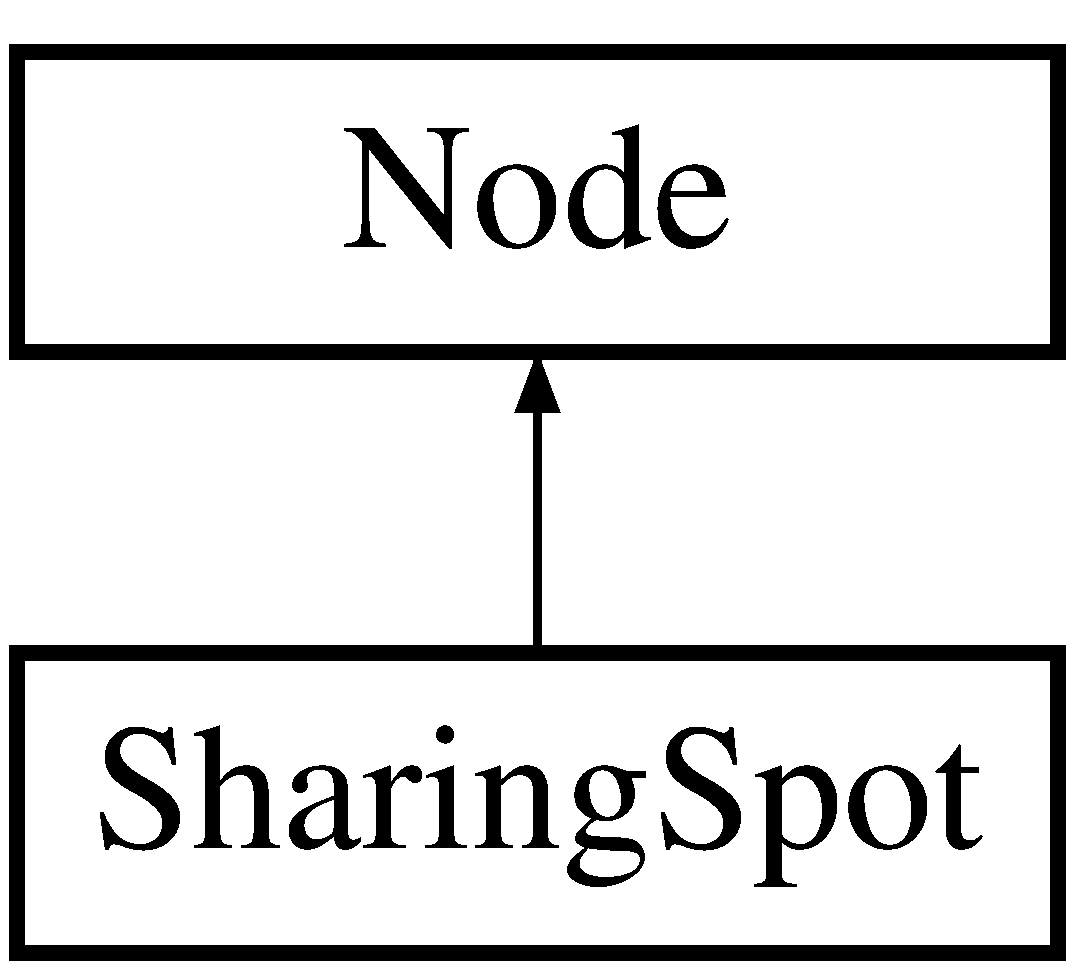
\includegraphics[height=2.000000cm]{class_node}
\end{center}
\end{figure}
\subsection*{Public Member Functions}
\begin{DoxyCompactItemize}
\item 
\mbox{\hyperlink{class_node_a082d5efb0be81faaeb35dc02b2a4fc76}{Node}} ()=default
\item 
\mbox{\hyperlink{class_node_af4abc294f8eadd6fbf4714150838c709}{Node}} (double latitude, double longitude)
\item 
unsigned int \mbox{\hyperlink{class_node_af9b4c1c72ce14b69f5e99deb4440f489}{get\+Id}} () const
\item 
double \mbox{\hyperlink{class_node_ad4a79ebbcca46dae4638ffbe4d732399}{get\+Longitude}} () const
\item 
double \mbox{\hyperlink{class_node_a6a76240688eddc8a2942618074e28c92}{get\+Latitude}} () const
\item 
bool \mbox{\hyperlink{class_node_ad5e2b0cf9850f22ac9668971f66759dc}{operator==}} (const \mbox{\hyperlink{class_node}{Node}} \&n2) const
\item 
double \mbox{\hyperlink{class_node_a765bf631776ac8efed4b5626582643ad}{calculate\+Distance}} (\mbox{\hyperlink{class_node}{Node}} \&n2)
\item 
void \mbox{\hyperlink{class_node_aafb92e93512d42b7f60bf18878003214}{add\+Street}} (int street\+ID)
\item 
const vector$<$ int $>$ \& \mbox{\hyperlink{class_node_ae96d5a45681f9d0517cf927514aec7f5}{get\+Streets}} () const
\item 
void \mbox{\hyperlink{class_node_a1c64b31b2afe1d39a10809da9198a016}{set\+Longitude}} (double longitude)
\item 
void \mbox{\hyperlink{class_node_ac62ad99961481d9e4b21dd4332717927}{set\+Latitude}} (double latitude)
\end{DoxyCompactItemize}
\subsection*{Static Public Attributes}
\begin{DoxyCompactItemize}
\item 
\mbox{\Hypertarget{class_node_ac862318be744cac98cdba7c7648a04d4}\label{class_node_ac862318be744cac98cdba7c7648a04d4}} 
static unsigned int {\bfseries count} = 1
\end{DoxyCompactItemize}
\subsection*{Protected Attributes}
\begin{DoxyCompactItemize}
\item 
\mbox{\Hypertarget{class_node_adb90577d9d796c4ccbccf41ce2efc6c9}\label{class_node_adb90577d9d796c4ccbccf41ce2efc6c9}} 
unsigned int {\bfseries id}
\item 
\mbox{\Hypertarget{class_node_af1772ed9e687d1e230f21c8fdf955ee9}\label{class_node_af1772ed9e687d1e230f21c8fdf955ee9}} 
double {\bfseries longitude}
\item 
\mbox{\Hypertarget{class_node_a18e537ee3be0b0f494e54d19486b532b}\label{class_node_a18e537ee3be0b0f494e54d19486b532b}} 
double {\bfseries latitude}
\item 
\mbox{\Hypertarget{class_node_ae028d72126fae2e69f65b230ef8b03ce}\label{class_node_ae028d72126fae2e69f65b230ef8b03ce}} 
vector$<$ int $>$ {\bfseries streets}
\end{DoxyCompactItemize}


\subsection{Detailed Description}
\mbox{\hyperlink{class_node}{Node}} class containing node information and a vector with the ids of the streets that pass throught it 

\subsection{Constructor \& Destructor Documentation}
\mbox{\Hypertarget{class_node_a082d5efb0be81faaeb35dc02b2a4fc76}\label{class_node_a082d5efb0be81faaeb35dc02b2a4fc76}} 
\index{Node@{Node}!Node@{Node}}
\index{Node@{Node}!Node@{Node}}
\subsubsection{\texorpdfstring{Node()}{Node()}\hspace{0.1cm}{\footnotesize\ttfamily [1/2]}}
{\footnotesize\ttfamily Node\+::\+Node (\begin{DoxyParamCaption}{ }\end{DoxyParamCaption})\hspace{0.3cm}{\ttfamily [default]}}

\mbox{\hyperlink{class_node}{Node}} default constructor \mbox{\Hypertarget{class_node_af4abc294f8eadd6fbf4714150838c709}\label{class_node_af4abc294f8eadd6fbf4714150838c709}} 
\index{Node@{Node}!Node@{Node}}
\index{Node@{Node}!Node@{Node}}
\subsubsection{\texorpdfstring{Node()}{Node()}\hspace{0.1cm}{\footnotesize\ttfamily [2/2]}}
{\footnotesize\ttfamily Node\+::\+Node (\begin{DoxyParamCaption}\item[{double}]{latitude,  }\item[{double}]{longitude }\end{DoxyParamCaption})}

\mbox{\hyperlink{class_node}{Node}} constructor 
\begin{DoxyParams}{Parameters}
{\em osm\+Id} & node osm id \\
\hline
{\em latitude} & node latitude \\
\hline
{\em longitude} & node longitude \\
\hline
\end{DoxyParams}


\subsection{Member Function Documentation}
\mbox{\Hypertarget{class_node_aafb92e93512d42b7f60bf18878003214}\label{class_node_aafb92e93512d42b7f60bf18878003214}} 
\index{Node@{Node}!add\+Street@{add\+Street}}
\index{add\+Street@{add\+Street}!Node@{Node}}
\subsubsection{\texorpdfstring{add\+Street()}{addStreet()}}
{\footnotesize\ttfamily void Node\+::add\+Street (\begin{DoxyParamCaption}\item[{int}]{street\+ID }\end{DoxyParamCaption})}

Adds a street ID do the node 
\begin{DoxyParams}{Parameters}
{\em int} & street id to be added \\
\hline
\end{DoxyParams}
\mbox{\Hypertarget{class_node_a765bf631776ac8efed4b5626582643ad}\label{class_node_a765bf631776ac8efed4b5626582643ad}} 
\index{Node@{Node}!calculate\+Distance@{calculate\+Distance}}
\index{calculate\+Distance@{calculate\+Distance}!Node@{Node}}
\subsubsection{\texorpdfstring{calculate\+Distance()}{calculateDistance()}}
{\footnotesize\ttfamily double Node\+::calculate\+Distance (\begin{DoxyParamCaption}\item[{\mbox{\hyperlink{class_node}{Node}} \&}]{n2 }\end{DoxyParamCaption})}

Calculates the distance between two nodes. 
\begin{DoxyParams}{Parameters}
{\em n2} & Second node. \\
\hline
\end{DoxyParams}
\begin{DoxyReturn}{Returns}
Distance between both nodes. 
\end{DoxyReturn}
\mbox{\Hypertarget{class_node_af9b4c1c72ce14b69f5e99deb4440f489}\label{class_node_af9b4c1c72ce14b69f5e99deb4440f489}} 
\index{Node@{Node}!get\+Id@{get\+Id}}
\index{get\+Id@{get\+Id}!Node@{Node}}
\subsubsection{\texorpdfstring{get\+Id()}{getId()}}
{\footnotesize\ttfamily unsigned int Node\+::get\+Id (\begin{DoxyParamCaption}{ }\end{DoxyParamCaption}) const}

Getter which returns the node id \begin{DoxyReturn}{Returns}
id 
\end{DoxyReturn}
\mbox{\Hypertarget{class_node_a6a76240688eddc8a2942618074e28c92}\label{class_node_a6a76240688eddc8a2942618074e28c92}} 
\index{Node@{Node}!get\+Latitude@{get\+Latitude}}
\index{get\+Latitude@{get\+Latitude}!Node@{Node}}
\subsubsection{\texorpdfstring{get\+Latitude()}{getLatitude()}}
{\footnotesize\ttfamily double Node\+::get\+Latitude (\begin{DoxyParamCaption}{ }\end{DoxyParamCaption}) const}

Getter which returns the node Latitude \begin{DoxyReturn}{Returns}
latitude 
\end{DoxyReturn}
\mbox{\Hypertarget{class_node_ad4a79ebbcca46dae4638ffbe4d732399}\label{class_node_ad4a79ebbcca46dae4638ffbe4d732399}} 
\index{Node@{Node}!get\+Longitude@{get\+Longitude}}
\index{get\+Longitude@{get\+Longitude}!Node@{Node}}
\subsubsection{\texorpdfstring{get\+Longitude()}{getLongitude()}}
{\footnotesize\ttfamily double Node\+::get\+Longitude (\begin{DoxyParamCaption}{ }\end{DoxyParamCaption}) const}

Getter which returns the node Longitude \begin{DoxyReturn}{Returns}
longitude 
\end{DoxyReturn}
\mbox{\Hypertarget{class_node_ae96d5a45681f9d0517cf927514aec7f5}\label{class_node_ae96d5a45681f9d0517cf927514aec7f5}} 
\index{Node@{Node}!get\+Streets@{get\+Streets}}
\index{get\+Streets@{get\+Streets}!Node@{Node}}
\subsubsection{\texorpdfstring{get\+Streets()}{getStreets()}}
{\footnotesize\ttfamily const vector$<$ int $>$ \& Node\+::get\+Streets (\begin{DoxyParamCaption}{ }\end{DoxyParamCaption}) const}

Getter for streets id \begin{DoxyReturn}{Returns}
street id vector 
\end{DoxyReturn}
\mbox{\Hypertarget{class_node_ad5e2b0cf9850f22ac9668971f66759dc}\label{class_node_ad5e2b0cf9850f22ac9668971f66759dc}} 
\index{Node@{Node}!operator==@{operator==}}
\index{operator==@{operator==}!Node@{Node}}
\subsubsection{\texorpdfstring{operator==()}{operator==()}}
{\footnotesize\ttfamily bool Node\+::operator== (\begin{DoxyParamCaption}\item[{const \mbox{\hyperlink{class_node}{Node}} \&}]{n2 }\end{DoxyParamCaption}) const}

Overload for the \textquotesingle{}==\textquotesingle{} operator for the \mbox{\hyperlink{class_node}{Node}} class 
\begin{DoxyParams}{Parameters}
{\em n2} & \mbox{\hyperlink{class_node}{Node}} to compare \\
\hline
\end{DoxyParams}
\begin{DoxyReturn}{Returns}
Returns true if both nodes have same id 
\end{DoxyReturn}
\mbox{\Hypertarget{class_node_ac62ad99961481d9e4b21dd4332717927}\label{class_node_ac62ad99961481d9e4b21dd4332717927}} 
\index{Node@{Node}!set\+Latitude@{set\+Latitude}}
\index{set\+Latitude@{set\+Latitude}!Node@{Node}}
\subsubsection{\texorpdfstring{set\+Latitude()}{setLatitude()}}
{\footnotesize\ttfamily void Node\+::set\+Latitude (\begin{DoxyParamCaption}\item[{double}]{latitude }\end{DoxyParamCaption})}

Setter for latitude 
\begin{DoxyParams}{Parameters}
{\em latitude} & latitude \\
\hline
\end{DoxyParams}
\mbox{\Hypertarget{class_node_a1c64b31b2afe1d39a10809da9198a016}\label{class_node_a1c64b31b2afe1d39a10809da9198a016}} 
\index{Node@{Node}!set\+Longitude@{set\+Longitude}}
\index{set\+Longitude@{set\+Longitude}!Node@{Node}}
\subsubsection{\texorpdfstring{set\+Longitude()}{setLongitude()}}
{\footnotesize\ttfamily void Node\+::set\+Longitude (\begin{DoxyParamCaption}\item[{double}]{longitude }\end{DoxyParamCaption})}

Setter for longitude 
\begin{DoxyParams}{Parameters}
{\em longitude} & longitude \\
\hline
\end{DoxyParams}


The documentation for this class was generated from the following files\+:\begin{DoxyCompactItemize}
\item 
src/Node.\+h\item 
src/Node.\+cpp\end{DoxyCompactItemize}

\hypertarget{class_parser}{}\section{Parser Class Reference}
\label{class_parser}\index{Parser@{Parser}}


{\ttfamily \#include $<$Parser.\+h$>$}

\subsection*{Public Member Functions}
\begin{DoxyCompactItemize}
\item 
\mbox{\Hypertarget{class_parser_a5208129b497bfdf7c8ecceeb70e4bba8}\label{class_parser_a5208129b497bfdf7c8ecceeb70e4bba8}} 
\mbox{\hyperlink{class_parser_a5208129b497bfdf7c8ecceeb70e4bba8}{Parser}} ()=default
\begin{DoxyCompactList}\small\item\em default constructor of a \mbox{\hyperlink{class_parser}{Parser}} object \end{DoxyCompactList}\item 
vector$<$ \mbox{\hyperlink{class_node}{Node}} $>$ \mbox{\hyperlink{class_parser_a6cb129a0533a784d9889fb522b3659f2}{read\+Nodes}} (string file)
\begin{DoxyCompactList}\small\item\em Returns a vector with all the nodes after being created from the data read from the file with the name passed as parameter. \end{DoxyCompactList}\item 
vector$<$ \mbox{\hyperlink{class_street}{Street}} $>$ \mbox{\hyperlink{class_parser_ac393c2185887253d615692ed871823f9}{read\+Streets}} (string file)
\begin{DoxyCompactList}\small\item\em Returns a vector with all the streets after being created from the data read from the file with the name passed as parameter. \end{DoxyCompactList}\item 
void \mbox{\hyperlink{class_parser_a67de76f90c398140fcc14c9ec7d8f00d}{read\+Relations}} (string file, vector$<$ \mbox{\hyperlink{class_street}{Street}} $>$ \&streets, vector$<$ \mbox{\hyperlink{class_node}{Node}} $>$ \&nodes, vector$<$ \mbox{\hyperlink{class_sharing_spot}{Sharing\+Spot}} $>$ \&spots)
\begin{DoxyCompactList}\small\item\em Reads the relations between streets and Nodes and uses that information to complete the streets and nodes objects already created. \end{DoxyCompactList}\item 
\mbox{\hyperlink{class_node}{Node}} \mbox{\hyperlink{class_parser_a69118b5346049a40a31eabcdbdbe1d4f}{create\+Node}} (string \&line)
\item 
\mbox{\hyperlink{class_street}{Street}} \mbox{\hyperlink{class_parser_a32dd986c0abb09bb1aaeb9683d3df616}{create\+Street}} (string \&line)
\item 
void \mbox{\hyperlink{class_parser_abc6f5fd0f2bf4a8ecca4b23c4a84d168}{create\+Relation}} (string \&line, vector$<$ \mbox{\hyperlink{class_street}{Street}} $>$ \&streets, vector$<$ \mbox{\hyperlink{class_node}{Node}} $>$ \&nodes, vector$<$ unsigned long long int $>$ \&streets\+ID)
\begin{DoxyCompactList}\small\item\em Analyzes a line from the Relations file and transforms that line into information to be put in Streets and Nodes. \end{DoxyCompactList}\item 
void \mbox{\hyperlink{class_parser_a4cd265d02c182e14a071407408468af0}{next}} (unsigned long long int \&elem, string \&piece, string separator)
\begin{DoxyCompactList}\small\item\em separates string based on the separator \end{DoxyCompactList}\item 
void \mbox{\hyperlink{class_parser_af2f740981e70de7602e8c2bcb3db904e}{next}} (double \&elem, string \&piece, string separator)
\begin{DoxyCompactList}\small\item\em separates string based on the separator \end{DoxyCompactList}\item 
void \mbox{\hyperlink{class_parser_a143c7f81ca7d3fb0a4013f8821126e0f}{next}} (string \&piece, string \&line, string separator)
\begin{DoxyCompactList}\small\item\em separates string based on the separator \end{DoxyCompactList}\item 
bool \mbox{\hyperlink{class_parser_ac49eaa953c8f063c8a3119b36df32c90}{valid\+String}} (string \&s)
\begin{DoxyCompactList}\small\item\em checks if input is valid \end{DoxyCompactList}\item 
void \mbox{\hyperlink{class_parser_a9b8221457783a9669e14ba266d976f6e}{create\+Sharing\+Spot}} (\mbox{\hyperlink{class_node}{Node}} n, vector$<$ \mbox{\hyperlink{class_sharing_spot}{Sharing\+Spot}} $>$ \&spots)
\begin{DoxyCompactList}\small\item\em creates a sharing spot \end{DoxyCompactList}\end{DoxyCompactItemize}


\subsection{Detailed Description}
\mbox{\hyperlink{class_parser}{Parser}} class containing the functions to parse the information from the files 

\subsection{Member Function Documentation}
\mbox{\Hypertarget{class_parser_a69118b5346049a40a31eabcdbdbe1d4f}\label{class_parser_a69118b5346049a40a31eabcdbdbe1d4f}} 
\index{Parser@{Parser}!create\+Node@{create\+Node}}
\index{create\+Node@{create\+Node}!Parser@{Parser}}
\subsubsection{\texorpdfstring{create\+Node()}{createNode()}}
{\footnotesize\ttfamily \mbox{\hyperlink{class_node}{Node}} Parser\+::create\+Node (\begin{DoxyParamCaption}\item[{string \&}]{line }\end{DoxyParamCaption})}

Auxiliary function that creates and returns a \mbox{\hyperlink{class_node}{Node}} based on the data in the line 
\begin{DoxyParams}{Parameters}
{\em line} & \\
\hline
\end{DoxyParams}
\begin{DoxyReturn}{Returns}
\mbox{\hyperlink{class_node}{Node}} 
\end{DoxyReturn}
\mbox{\Hypertarget{class_parser_abc6f5fd0f2bf4a8ecca4b23c4a84d168}\label{class_parser_abc6f5fd0f2bf4a8ecca4b23c4a84d168}} 
\index{Parser@{Parser}!create\+Relation@{create\+Relation}}
\index{create\+Relation@{create\+Relation}!Parser@{Parser}}
\subsubsection{\texorpdfstring{create\+Relation()}{createRelation()}}
{\footnotesize\ttfamily void Parser\+::create\+Relation (\begin{DoxyParamCaption}\item[{string \&}]{line,  }\item[{vector$<$ \mbox{\hyperlink{class_street}{Street}} $>$ \&}]{streets,  }\item[{vector$<$ \mbox{\hyperlink{class_node}{Node}} $>$ \&}]{nodes,  }\item[{vector$<$ unsigned long long int $>$ \&}]{streets\+ID }\end{DoxyParamCaption})}



Analyzes a line from the Relations file and transforms that line into information to be put in Streets and Nodes. 


\begin{DoxyParams}{Parameters}
{\em line} & string \\
\hline
{\em streets} & vector $<$\+Street$>$ \\
\hline
{\em nodes} & vector $<$\+Node$>$ \\
\hline
{\em streets\+ID} & vector $<$int$>$ \\
\hline
\end{DoxyParams}
\mbox{\Hypertarget{class_parser_a9b8221457783a9669e14ba266d976f6e}\label{class_parser_a9b8221457783a9669e14ba266d976f6e}} 
\index{Parser@{Parser}!create\+Sharing\+Spot@{create\+Sharing\+Spot}}
\index{create\+Sharing\+Spot@{create\+Sharing\+Spot}!Parser@{Parser}}
\subsubsection{\texorpdfstring{create\+Sharing\+Spot()}{createSharingSpot()}}
{\footnotesize\ttfamily void Parser\+::create\+Sharing\+Spot (\begin{DoxyParamCaption}\item[{\mbox{\hyperlink{class_node}{Node}}}]{n,  }\item[{vector$<$ \mbox{\hyperlink{class_sharing_spot}{Sharing\+Spot}} $>$ \&}]{spots }\end{DoxyParamCaption})}



creates a sharing spot 


\begin{DoxyParams}{Parameters}
{\em n} & node that will be a sharing spot \\
\hline
{\em spots} & sharing spot vector to add the sharing spot \\
\hline
\end{DoxyParams}
\mbox{\Hypertarget{class_parser_a32dd986c0abb09bb1aaeb9683d3df616}\label{class_parser_a32dd986c0abb09bb1aaeb9683d3df616}} 
\index{Parser@{Parser}!create\+Street@{create\+Street}}
\index{create\+Street@{create\+Street}!Parser@{Parser}}
\subsubsection{\texorpdfstring{create\+Street()}{createStreet()}}
{\footnotesize\ttfamily \mbox{\hyperlink{class_street}{Street}} Parser\+::create\+Street (\begin{DoxyParamCaption}\item[{string \&}]{line }\end{DoxyParamCaption})}

Auxiliary function that creates and returns a \mbox{\hyperlink{class_street}{Street}} based on the data in the line 
\begin{DoxyParams}{Parameters}
{\em line} & \\
\hline
\end{DoxyParams}
\begin{DoxyReturn}{Returns}
\mbox{\hyperlink{class_street}{Street}} 
\end{DoxyReturn}
\mbox{\Hypertarget{class_parser_a4cd265d02c182e14a071407408468af0}\label{class_parser_a4cd265d02c182e14a071407408468af0}} 
\index{Parser@{Parser}!next@{next}}
\index{next@{next}!Parser@{Parser}}
\subsubsection{\texorpdfstring{next()}{next()}\hspace{0.1cm}{\footnotesize\ttfamily [1/3]}}
{\footnotesize\ttfamily void Parser\+::next (\begin{DoxyParamCaption}\item[{unsigned long long int \&}]{elem,  }\item[{string \&}]{piece,  }\item[{string}]{separator }\end{DoxyParamCaption})}



separates string based on the separator 


\begin{DoxyParams}{Parameters}
{\em elem} & unsigned long long int \&elem \\
\hline
{\em piece} & string \&piece \\
\hline
{\em separator} & string separator \\
\hline
\end{DoxyParams}
\mbox{\Hypertarget{class_parser_af2f740981e70de7602e8c2bcb3db904e}\label{class_parser_af2f740981e70de7602e8c2bcb3db904e}} 
\index{Parser@{Parser}!next@{next}}
\index{next@{next}!Parser@{Parser}}
\subsubsection{\texorpdfstring{next()}{next()}\hspace{0.1cm}{\footnotesize\ttfamily [2/3]}}
{\footnotesize\ttfamily void Parser\+::next (\begin{DoxyParamCaption}\item[{double \&}]{elem,  }\item[{string \&}]{piece,  }\item[{string}]{separator }\end{DoxyParamCaption})}



separates string based on the separator 


\begin{DoxyParams}{Parameters}
{\em elem} & double \&elem \\
\hline
{\em piece} & string \&piece \\
\hline
{\em separator} & string separator \\
\hline
\end{DoxyParams}
\mbox{\Hypertarget{class_parser_a143c7f81ca7d3fb0a4013f8821126e0f}\label{class_parser_a143c7f81ca7d3fb0a4013f8821126e0f}} 
\index{Parser@{Parser}!next@{next}}
\index{next@{next}!Parser@{Parser}}
\subsubsection{\texorpdfstring{next()}{next()}\hspace{0.1cm}{\footnotesize\ttfamily [3/3]}}
{\footnotesize\ttfamily void Parser\+::next (\begin{DoxyParamCaption}\item[{string \&}]{piece,  }\item[{string \&}]{line,  }\item[{string}]{separator }\end{DoxyParamCaption})}



separates string based on the separator 


\begin{DoxyParams}{Parameters}
{\em piece} & \\
\hline
{\em line} & \\
\hline
{\em separator} & \\
\hline
\end{DoxyParams}
\mbox{\Hypertarget{class_parser_a6cb129a0533a784d9889fb522b3659f2}\label{class_parser_a6cb129a0533a784d9889fb522b3659f2}} 
\index{Parser@{Parser}!read\+Nodes@{read\+Nodes}}
\index{read\+Nodes@{read\+Nodes}!Parser@{Parser}}
\subsubsection{\texorpdfstring{read\+Nodes()}{readNodes()}}
{\footnotesize\ttfamily vector$<$ \mbox{\hyperlink{class_node}{Node}} $>$ Parser\+::read\+Nodes (\begin{DoxyParamCaption}\item[{string}]{file }\end{DoxyParamCaption})}



Returns a vector with all the nodes after being created from the data read from the file with the name passed as parameter. 


\begin{DoxyParams}{Parameters}
{\em file} & string \\
\hline
\end{DoxyParams}
\begin{DoxyReturn}{Returns}
vector $<$\+Node$>$ 
\end{DoxyReturn}
\mbox{\Hypertarget{class_parser_a67de76f90c398140fcc14c9ec7d8f00d}\label{class_parser_a67de76f90c398140fcc14c9ec7d8f00d}} 
\index{Parser@{Parser}!read\+Relations@{read\+Relations}}
\index{read\+Relations@{read\+Relations}!Parser@{Parser}}
\subsubsection{\texorpdfstring{read\+Relations()}{readRelations()}}
{\footnotesize\ttfamily void Parser\+::read\+Relations (\begin{DoxyParamCaption}\item[{string}]{file,  }\item[{vector$<$ \mbox{\hyperlink{class_street}{Street}} $>$ \&}]{streets,  }\item[{vector$<$ \mbox{\hyperlink{class_node}{Node}} $>$ \&}]{nodes,  }\item[{vector$<$ \mbox{\hyperlink{class_sharing_spot}{Sharing\+Spot}} $>$ \&}]{spots }\end{DoxyParamCaption})}



Reads the relations between streets and Nodes and uses that information to complete the streets and nodes objects already created. 


\begin{DoxyParams}{Parameters}
{\em file} & string \\
\hline
{\em streets} & vector $<$\+Street$>$ \\
\hline
{\em nodes} & vector $<$\+Node$>$ \\
\hline
\end{DoxyParams}
\mbox{\Hypertarget{class_parser_ac393c2185887253d615692ed871823f9}\label{class_parser_ac393c2185887253d615692ed871823f9}} 
\index{Parser@{Parser}!read\+Streets@{read\+Streets}}
\index{read\+Streets@{read\+Streets}!Parser@{Parser}}
\subsubsection{\texorpdfstring{read\+Streets()}{readStreets()}}
{\footnotesize\ttfamily vector$<$ \mbox{\hyperlink{class_street}{Street}} $>$ Parser\+::read\+Streets (\begin{DoxyParamCaption}\item[{string}]{file }\end{DoxyParamCaption})}



Returns a vector with all the streets after being created from the data read from the file with the name passed as parameter. 


\begin{DoxyParams}{Parameters}
{\em file} & string \\
\hline
\end{DoxyParams}
\begin{DoxyReturn}{Returns}
vector $<$\+Street$>$ 
\end{DoxyReturn}
\mbox{\Hypertarget{class_parser_ac49eaa953c8f063c8a3119b36df32c90}\label{class_parser_ac49eaa953c8f063c8a3119b36df32c90}} 
\index{Parser@{Parser}!valid\+String@{valid\+String}}
\index{valid\+String@{valid\+String}!Parser@{Parser}}
\subsubsection{\texorpdfstring{valid\+String()}{validString()}}
{\footnotesize\ttfamily bool Parser\+::valid\+String (\begin{DoxyParamCaption}\item[{string \&}]{s }\end{DoxyParamCaption})}



checks if input is valid 


\begin{DoxyParams}{Parameters}
{\em s} & string \&s \\
\hline
\end{DoxyParams}
\begin{DoxyReturn}{Returns}
true if input is valid and false otherwise 
\end{DoxyReturn}


The documentation for this class was generated from the following files\+:\begin{DoxyCompactItemize}
\item 
src/Parser.\+h\item 
src/Parser.\+cpp\end{DoxyCompactItemize}

\hypertarget{class_sharing_spot}{}\section{Sharing\+Spot Class Reference}
\label{class_sharing_spot}\index{Sharing\+Spot@{Sharing\+Spot}}


{\ttfamily \#include $<$Sharing\+Spot.\+h$>$}

Inheritance diagram for Sharing\+Spot\+:\begin{figure}[H]
\begin{center}
\leavevmode
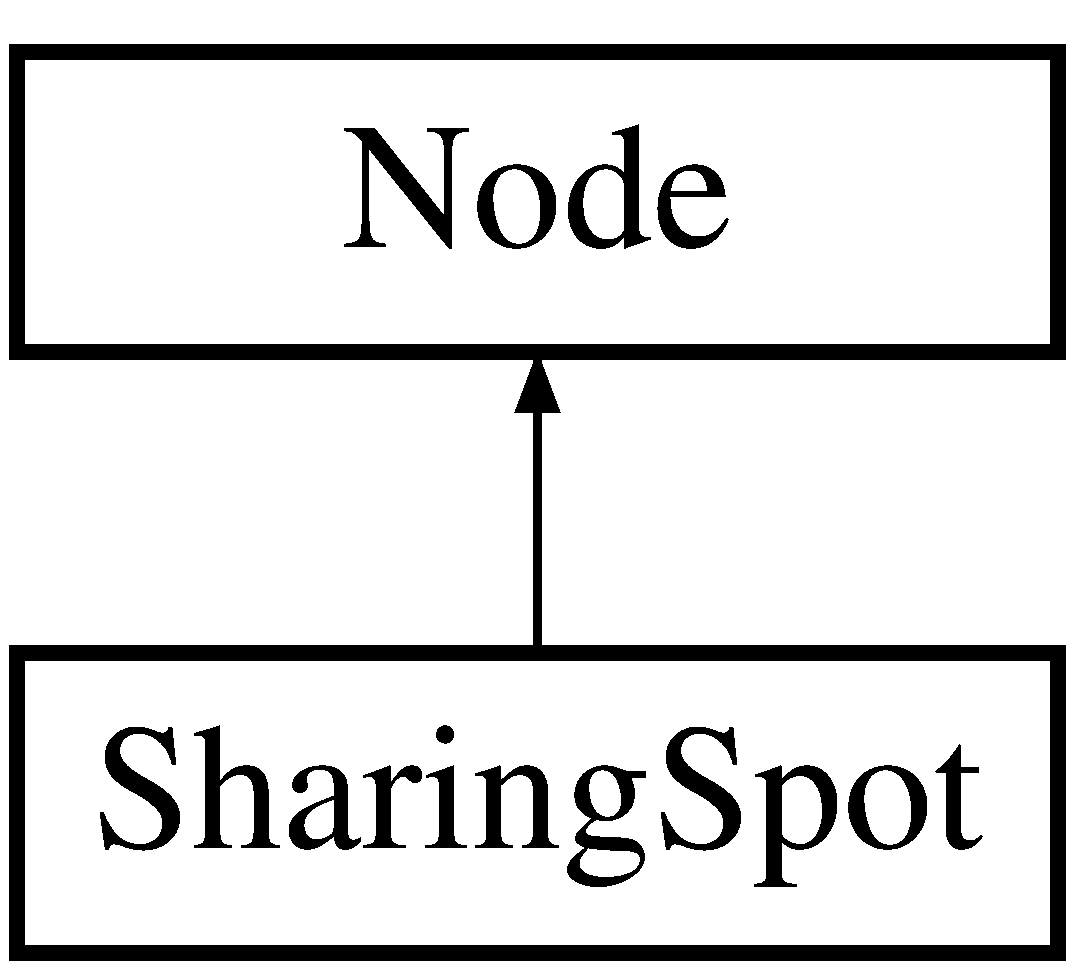
\includegraphics[height=2.000000cm]{class_sharing_spot}
\end{center}
\end{figure}
\subsection*{Public Member Functions}
\begin{DoxyCompactItemize}
\item 
\mbox{\hyperlink{class_sharing_spot_a1110d1c6955a7aa434a87bffb32e2ea3}{Sharing\+Spot}} (\mbox{\hyperlink{class_node}{Node}} n)
\item 
bool \mbox{\hyperlink{class_sharing_spot_a6b565d3a7fb62fb3235794a8381f9873}{is\+Free\+Spot}} () const
\end{DoxyCompactItemize}
\subsection*{Additional Inherited Members}


\subsection{Detailed Description}
Sharing Spot class derived from the node class, has a flag to check if it is free or not 

\subsection{Constructor \& Destructor Documentation}
\mbox{\Hypertarget{class_sharing_spot_a1110d1c6955a7aa434a87bffb32e2ea3}\label{class_sharing_spot_a1110d1c6955a7aa434a87bffb32e2ea3}} 
\index{Sharing\+Spot@{Sharing\+Spot}!Sharing\+Spot@{Sharing\+Spot}}
\index{Sharing\+Spot@{Sharing\+Spot}!Sharing\+Spot@{Sharing\+Spot}}
\subsubsection{\texorpdfstring{Sharing\+Spot()}{SharingSpot()}}
{\footnotesize\ttfamily Sharing\+Spot\+::\+Sharing\+Spot (\begin{DoxyParamCaption}\item[{\mbox{\hyperlink{class_node}{Node}}}]{n }\end{DoxyParamCaption})\hspace{0.3cm}{\ttfamily [explicit]}}

Sharing spot constructor (whether it is free or not is calculated here) 
\begin{DoxyParams}{Parameters}
{\em n} & node where the sharing spot will be placed \\
\hline
\end{DoxyParams}


\subsection{Member Function Documentation}
\mbox{\Hypertarget{class_sharing_spot_a6b565d3a7fb62fb3235794a8381f9873}\label{class_sharing_spot_a6b565d3a7fb62fb3235794a8381f9873}} 
\index{Sharing\+Spot@{Sharing\+Spot}!is\+Free\+Spot@{is\+Free\+Spot}}
\index{is\+Free\+Spot@{is\+Free\+Spot}!Sharing\+Spot@{Sharing\+Spot}}
\subsubsection{\texorpdfstring{is\+Free\+Spot()}{isFreeSpot()}}
{\footnotesize\ttfamily bool Sharing\+Spot\+::is\+Free\+Spot (\begin{DoxyParamCaption}{ }\end{DoxyParamCaption}) const}

Getter which returns wether the sharing spot is free or not \begin{DoxyReturn}{Returns}
if the spot is free or not 
\end{DoxyReturn}


The documentation for this class was generated from the following files\+:\begin{DoxyCompactItemize}
\item 
src/Sharing\+Spot.\+h\item 
src/Sharing\+Spot.\+cpp\end{DoxyCompactItemize}

\hypertarget{class_street}{}\section{Street Class Reference}
\label{class_street}\index{Street@{Street}}


{\ttfamily \#include $<$Street.\+h$>$}

\subsection*{Public Member Functions}
\begin{DoxyCompactItemize}
\item 
\mbox{\hyperlink{class_street_a67c6b12ed40488038123d2798586a49a}{Street}} ()
\item 
\mbox{\hyperlink{class_street_a5a9d10bd309a37eebd309aefb678f2fc}{Street}} (string \&name, bool two\+Ways, int elevation)
\item 
unsigned int \mbox{\hyperlink{class_street_af5bd31425eba6d72a3c81505e720249b}{get\+Id}} () const
\item 
const string \& \mbox{\hyperlink{class_street_afcd581ec643416f80695460ca8c19c73}{get\+Name}} () const
\item 
bool \mbox{\hyperlink{class_street_a2948b1e4a058de686bd24af9fe5fa1e0}{is\+Two\+Ways}} () const
\item 
void \mbox{\hyperlink{class_street_a6539789494cff71ffab2913bbb84f7cf}{set\+Two\+Ways}} (bool two\+Ways)
\item 
double \mbox{\hyperlink{class_street_af96504bfc1730a64fec877bb08125460}{get\+Elevation}} ()
\item 
void \mbox{\hyperlink{class_street_a17e7f3ac9efd4a137e2611ae945c4c03}{set\+Elevation}} (double elevation)
\item 
bool \mbox{\hyperlink{class_street_af902ded011ecdcec196873016bfe310e}{operator==}} (const \mbox{\hyperlink{class_street}{Street}} \&s2) const
\item 
void \mbox{\hyperlink{class_street_aded0fceaaa71f5cc8223296ec7489ac7}{add\+Node}} (\mbox{\hyperlink{class_node}{Node}} \&n)
\begin{DoxyCompactList}\small\item\em Adds de node passed as parameter to the \mbox{\hyperlink{class_street}{Street}} object. \end{DoxyCompactList}\item 
vector$<$ \mbox{\hyperlink{class_node}{Node}} $>$ \& \mbox{\hyperlink{class_street_afedbedacf271f93b5105708e1afc6be6}{get\+Nodes}} ()
\begin{DoxyCompactList}\small\item\em Getter which returns the vector of Nodes in a \mbox{\hyperlink{class_street}{Street}} object. \end{DoxyCompactList}\item 
int \mbox{\hyperlink{class_street_aa35e1a8c37690c9463edc97a1d0fe60e}{find\+Node}} (unsigned long long int id)
\item 
void \mbox{\hyperlink{class_street_ad93a7342b4be921e878f60b71f2d79f9}{add\+Street\+To\+Node}} (int i, int id)
\end{DoxyCompactItemize}
\subsection*{Static Public Attributes}
\begin{DoxyCompactItemize}
\item 
\mbox{\Hypertarget{class_street_aea6a60e70d589d29492fec22554cc513}\label{class_street_aea6a60e70d589d29492fec22554cc513}} 
static unsigned int {\bfseries count} = 1
\end{DoxyCompactItemize}


\subsection{Detailed Description}
\mbox{\hyperlink{class_street}{Street}} class containing all of the street info and a vector with all the nodes in it ordered 

\subsection{Constructor \& Destructor Documentation}
\mbox{\Hypertarget{class_street_a67c6b12ed40488038123d2798586a49a}\label{class_street_a67c6b12ed40488038123d2798586a49a}} 
\index{Street@{Street}!Street@{Street}}
\index{Street@{Street}!Street@{Street}}
\subsubsection{\texorpdfstring{Street()}{Street()}\hspace{0.1cm}{\footnotesize\ttfamily [1/2]}}
{\footnotesize\ttfamily Street\+::\+Street (\begin{DoxyParamCaption}{ }\end{DoxyParamCaption})\hspace{0.3cm}{\ttfamily [explicit]}}

\mbox{\hyperlink{class_street}{Street}} constructor with id \mbox{\Hypertarget{class_street_a5a9d10bd309a37eebd309aefb678f2fc}\label{class_street_a5a9d10bd309a37eebd309aefb678f2fc}} 
\index{Street@{Street}!Street@{Street}}
\index{Street@{Street}!Street@{Street}}
\subsubsection{\texorpdfstring{Street()}{Street()}\hspace{0.1cm}{\footnotesize\ttfamily [2/2]}}
{\footnotesize\ttfamily Street\+::\+Street (\begin{DoxyParamCaption}\item[{string \&}]{name,  }\item[{bool}]{two\+Ways,  }\item[{int}]{elevation }\end{DoxyParamCaption})}

\mbox{\hyperlink{class_street}{Street}} constructor where the slope is randomly calculated 
\begin{DoxyParams}{Parameters}
{\em elevation} & int elevation \\
\hline
{\em name} & street name \\
\hline
{\em two\+Ways} & flag that checks if the street is both ways \\
\hline
\end{DoxyParams}


\subsection{Member Function Documentation}
\mbox{\Hypertarget{class_street_aded0fceaaa71f5cc8223296ec7489ac7}\label{class_street_aded0fceaaa71f5cc8223296ec7489ac7}} 
\index{Street@{Street}!add\+Node@{add\+Node}}
\index{add\+Node@{add\+Node}!Street@{Street}}
\subsubsection{\texorpdfstring{add\+Node()}{addNode()}}
{\footnotesize\ttfamily void Street\+::add\+Node (\begin{DoxyParamCaption}\item[{\mbox{\hyperlink{class_node}{Node}} \&}]{n }\end{DoxyParamCaption})}



Adds de node passed as parameter to the \mbox{\hyperlink{class_street}{Street}} object. 


\begin{DoxyParams}{Parameters}
{\em n} & \mbox{\hyperlink{class_node}{Node}} to add \\
\hline
\end{DoxyParams}
\mbox{\Hypertarget{class_street_ad93a7342b4be921e878f60b71f2d79f9}\label{class_street_ad93a7342b4be921e878f60b71f2d79f9}} 
\index{Street@{Street}!add\+Street\+To\+Node@{add\+Street\+To\+Node}}
\index{add\+Street\+To\+Node@{add\+Street\+To\+Node}!Street@{Street}}
\subsubsection{\texorpdfstring{add\+Street\+To\+Node()}{addStreetToNode()}}
{\footnotesize\ttfamily void Street\+::add\+Street\+To\+Node (\begin{DoxyParamCaption}\item[{int}]{i,  }\item[{int}]{id }\end{DoxyParamCaption})}

add street to a node 
\begin{DoxyParams}{Parameters}
{\em i} & node index \\
\hline
{\em id} & street id \\
\hline
\end{DoxyParams}
\mbox{\Hypertarget{class_street_aa35e1a8c37690c9463edc97a1d0fe60e}\label{class_street_aa35e1a8c37690c9463edc97a1d0fe60e}} 
\index{Street@{Street}!find\+Node@{find\+Node}}
\index{find\+Node@{find\+Node}!Street@{Street}}
\subsubsection{\texorpdfstring{find\+Node()}{findNode()}}
{\footnotesize\ttfamily int Street\+::find\+Node (\begin{DoxyParamCaption}\item[{unsigned long long int}]{id }\end{DoxyParamCaption})}

finds the index of the node with the specified id 
\begin{DoxyParams}{Parameters}
{\em id} & node id \\
\hline
\end{DoxyParams}
\begin{DoxyReturn}{Returns}
returns node index 
\end{DoxyReturn}
\mbox{\Hypertarget{class_street_af96504bfc1730a64fec877bb08125460}\label{class_street_af96504bfc1730a64fec877bb08125460}} 
\index{Street@{Street}!get\+Elevation@{get\+Elevation}}
\index{get\+Elevation@{get\+Elevation}!Street@{Street}}
\subsubsection{\texorpdfstring{get\+Elevation()}{getElevation()}}
{\footnotesize\ttfamily double Street\+::get\+Elevation (\begin{DoxyParamCaption}{ }\end{DoxyParamCaption})}

Getter which returns the street elevation \begin{DoxyReturn}{Returns}
elevation double 
\end{DoxyReturn}
\mbox{\Hypertarget{class_street_af5bd31425eba6d72a3c81505e720249b}\label{class_street_af5bd31425eba6d72a3c81505e720249b}} 
\index{Street@{Street}!get\+Id@{get\+Id}}
\index{get\+Id@{get\+Id}!Street@{Street}}
\subsubsection{\texorpdfstring{get\+Id()}{getId()}}
{\footnotesize\ttfamily unsigned int Street\+::get\+Id (\begin{DoxyParamCaption}{ }\end{DoxyParamCaption}) const}

Getter which returns the street id \begin{DoxyReturn}{Returns}
id 
\end{DoxyReturn}
\mbox{\Hypertarget{class_street_afcd581ec643416f80695460ca8c19c73}\label{class_street_afcd581ec643416f80695460ca8c19c73}} 
\index{Street@{Street}!get\+Name@{get\+Name}}
\index{get\+Name@{get\+Name}!Street@{Street}}
\subsubsection{\texorpdfstring{get\+Name()}{getName()}}
{\footnotesize\ttfamily const string \& Street\+::get\+Name (\begin{DoxyParamCaption}{ }\end{DoxyParamCaption}) const}

Getter which returns the street name \begin{DoxyReturn}{Returns}
name 
\end{DoxyReturn}
\mbox{\Hypertarget{class_street_afedbedacf271f93b5105708e1afc6be6}\label{class_street_afedbedacf271f93b5105708e1afc6be6}} 
\index{Street@{Street}!get\+Nodes@{get\+Nodes}}
\index{get\+Nodes@{get\+Nodes}!Street@{Street}}
\subsubsection{\texorpdfstring{get\+Nodes()}{getNodes()}}
{\footnotesize\ttfamily vector$<$ \mbox{\hyperlink{class_node}{Node}} $>$ \& Street\+::get\+Nodes (\begin{DoxyParamCaption}{ }\end{DoxyParamCaption})}



Getter which returns the vector of Nodes in a \mbox{\hyperlink{class_street}{Street}} object. 

\begin{DoxyReturn}{Returns}
vector $<$\+Node$>$ 
\end{DoxyReturn}
\mbox{\Hypertarget{class_street_a2948b1e4a058de686bd24af9fe5fa1e0}\label{class_street_a2948b1e4a058de686bd24af9fe5fa1e0}} 
\index{Street@{Street}!is\+Two\+Ways@{is\+Two\+Ways}}
\index{is\+Two\+Ways@{is\+Two\+Ways}!Street@{Street}}
\subsubsection{\texorpdfstring{is\+Two\+Ways()}{isTwoWays()}}
{\footnotesize\ttfamily bool Street\+::is\+Two\+Ways (\begin{DoxyParamCaption}{ }\end{DoxyParamCaption}) const}

Getter which returns the flag that says if the street is both ways \begin{DoxyReturn}{Returns}
two ways flag 
\end{DoxyReturn}
\mbox{\Hypertarget{class_street_af902ded011ecdcec196873016bfe310e}\label{class_street_af902ded011ecdcec196873016bfe310e}} 
\index{Street@{Street}!operator==@{operator==}}
\index{operator==@{operator==}!Street@{Street}}
\subsubsection{\texorpdfstring{operator==()}{operator==()}}
{\footnotesize\ttfamily bool Street\+::operator== (\begin{DoxyParamCaption}\item[{const \mbox{\hyperlink{class_street}{Street}} \&}]{s2 }\end{DoxyParamCaption}) const}

Overload for the \textquotesingle{}==\textquotesingle{} operator for the \mbox{\hyperlink{class_street}{Street}} class 
\begin{DoxyParams}{Parameters}
{\em s2} & \mbox{\hyperlink{class_street}{Street}} to compare \\
\hline
\end{DoxyParams}
\begin{DoxyReturn}{Returns}
Returns true if both streets have same id 
\end{DoxyReturn}
\mbox{\Hypertarget{class_street_a17e7f3ac9efd4a137e2611ae945c4c03}\label{class_street_a17e7f3ac9efd4a137e2611ae945c4c03}} 
\index{Street@{Street}!set\+Elevation@{set\+Elevation}}
\index{set\+Elevation@{set\+Elevation}!Street@{Street}}
\subsubsection{\texorpdfstring{set\+Elevation()}{setElevation()}}
{\footnotesize\ttfamily void Street\+::set\+Elevation (\begin{DoxyParamCaption}\item[{double}]{elevation }\end{DoxyParamCaption})}

Setter which sets the street elevation 
\begin{DoxyParams}{Parameters}
{\em elevation} & double elevation to be set on the \mbox{\hyperlink{class_street}{Street}} object \\
\hline
\end{DoxyParams}
\mbox{\Hypertarget{class_street_a6539789494cff71ffab2913bbb84f7cf}\label{class_street_a6539789494cff71ffab2913bbb84f7cf}} 
\index{Street@{Street}!set\+Two\+Ways@{set\+Two\+Ways}}
\index{set\+Two\+Ways@{set\+Two\+Ways}!Street@{Street}}
\subsubsection{\texorpdfstring{set\+Two\+Ways()}{setTwoWays()}}
{\footnotesize\ttfamily void Street\+::set\+Two\+Ways (\begin{DoxyParamCaption}\item[{bool}]{two\+Ways }\end{DoxyParamCaption})}

Setter which sets the two\+Ways flag 
\begin{DoxyParams}{Parameters}
{\em two\+Ways} & value to wich the two\+Ways flag will be changed \\
\hline
\end{DoxyParams}


The documentation for this class was generated from the following files\+:\begin{DoxyCompactItemize}
\item 
src/Street.\+h\item 
src/Street.\+cpp\end{DoxyCompactItemize}

\hypertarget{class_user}{}\section{User Class Reference}
\label{class_user}\index{User@{User}}
\subsection*{Public Member Functions}
\begin{DoxyCompactItemize}
\item 
\mbox{\hyperlink{class_user_a4dd5fde1b81bb132994a67f27bc203d1}{User}} ()=default
\item 
\mbox{\hyperlink{class_user_ad4a962e2a4725118c5ea7a5af8362a66}{User}} (Payment\+Method payment\+Method, string payment\+Information)
\item 
const Payment\+Method \& \mbox{\hyperlink{class_user_a7945c31f5147c86e9577a8500ac51b8e}{get\+Payment\+Method}} () const
\item 
const string \& \mbox{\hyperlink{class_user_a815ed7790a21f851257aea04bbd43881}{get\+Payment\+Information}} () const
\end{DoxyCompactItemize}


\subsection{Constructor \& Destructor Documentation}
\mbox{\Hypertarget{class_user_a4dd5fde1b81bb132994a67f27bc203d1}\label{class_user_a4dd5fde1b81bb132994a67f27bc203d1}} 
\index{User@{User}!User@{User}}
\index{User@{User}!User@{User}}
\subsubsection{\texorpdfstring{User()}{User()}\hspace{0.1cm}{\footnotesize\ttfamily [1/2]}}
{\footnotesize\ttfamily User\+::\+User (\begin{DoxyParamCaption}{ }\end{DoxyParamCaption})\hspace{0.3cm}{\ttfamily [default]}}

\mbox{\hyperlink{class_user}{User}} default constructor \mbox{\Hypertarget{class_user_ad4a962e2a4725118c5ea7a5af8362a66}\label{class_user_ad4a962e2a4725118c5ea7a5af8362a66}} 
\index{User@{User}!User@{User}}
\index{User@{User}!User@{User}}
\subsubsection{\texorpdfstring{User()}{User()}\hspace{0.1cm}{\footnotesize\ttfamily [2/2]}}
{\footnotesize\ttfamily User\+::\+User (\begin{DoxyParamCaption}\item[{Payment\+Method}]{payment\+Method,  }\item[{string}]{payment\+Information }\end{DoxyParamCaption})}

\mbox{\hyperlink{class_user}{User}} constructor 
\begin{DoxyParams}{Parameters}
{\em payment\+Method} & payment method \\
\hline
{\em payment\+Information} & payment information(creditcard number or paypal email) \\
\hline
\end{DoxyParams}


\subsection{Member Function Documentation}
\mbox{\Hypertarget{class_user_a815ed7790a21f851257aea04bbd43881}\label{class_user_a815ed7790a21f851257aea04bbd43881}} 
\index{User@{User}!get\+Payment\+Information@{get\+Payment\+Information}}
\index{get\+Payment\+Information@{get\+Payment\+Information}!User@{User}}
\subsubsection{\texorpdfstring{get\+Payment\+Information()}{getPaymentInformation()}}
{\footnotesize\ttfamily const string \& User\+::get\+Payment\+Information (\begin{DoxyParamCaption}{ }\end{DoxyParamCaption}) const}

Getter which returns the payment information (creditcard number or paypal email) \begin{DoxyReturn}{Returns}
payment information 
\end{DoxyReturn}
\mbox{\Hypertarget{class_user_a7945c31f5147c86e9577a8500ac51b8e}\label{class_user_a7945c31f5147c86e9577a8500ac51b8e}} 
\index{User@{User}!get\+Payment\+Method@{get\+Payment\+Method}}
\index{get\+Payment\+Method@{get\+Payment\+Method}!User@{User}}
\subsubsection{\texorpdfstring{get\+Payment\+Method()}{getPaymentMethod()}}
{\footnotesize\ttfamily const Payment\+Method \& User\+::get\+Payment\+Method (\begin{DoxyParamCaption}{ }\end{DoxyParamCaption}) const}

Getter which returns the payment method \begin{DoxyReturn}{Returns}
payment method 
\end{DoxyReturn}


The documentation for this class was generated from the following files\+:\begin{DoxyCompactItemize}
\item 
src/User.\+h\item 
src/User.\+cpp\end{DoxyCompactItemize}

\hypertarget{class_vertex}{}\section{Vertex$<$ T $>$ Class Template Reference}
\label{class_vertex}\index{Vertex$<$ T $>$@{Vertex$<$ T $>$}}
\subsection*{Public Member Functions}
\begin{DoxyCompactItemize}
\item 
\mbox{\Hypertarget{class_vertex_afcbdd4d4198b672356559cb8fa088408}\label{class_vertex_afcbdd4d4198b672356559cb8fa088408}} 
{\bfseries Vertex} (T in)
\item 
\mbox{\Hypertarget{class_vertex_a5a6670b842354232bac4dad2f551d66e}\label{class_vertex_a5a6670b842354232bac4dad2f551d66e}} 
bool {\bfseries operator$<$} (\mbox{\hyperlink{class_vertex}{Vertex}}$<$ T $>$ \&vertex) const
\item 
\mbox{\Hypertarget{class_vertex_a2d06d0997dd56735bad8baa45f45d3a0}\label{class_vertex_a2d06d0997dd56735bad8baa45f45d3a0}} 
double {\bfseries get\+Dist} ()
\end{DoxyCompactItemize}
\subsection*{Friends}
\begin{DoxyCompactItemize}
\item 
\mbox{\Hypertarget{class_vertex_aefa9b76cd57411c5354e5620dc2d84dd}\label{class_vertex_aefa9b76cd57411c5354e5620dc2d84dd}} 
class {\bfseries Graph$<$ T $>$}
\item 
\mbox{\Hypertarget{class_vertex_ae53e0b4fec14b9f1eaa8a4f8cd426e9e}\label{class_vertex_ae53e0b4fec14b9f1eaa8a4f8cd426e9e}} 
class {\bfseries Mutable\+Priority\+Queue$<$ Vertex$<$ T $>$ $>$}
\end{DoxyCompactItemize}


The documentation for this class was generated from the following file\+:\begin{DoxyCompactItemize}
\item 
src/graph.\+h\end{DoxyCompactItemize}

%--- End generated contents ---

% Index
\backmatter
\newpage
\phantomsection
\clearemptydoublepage
\addcontentsline{toc}{chapter}{Index}
\printindex

\end{document}
